% Merged preprint: new narrative framework + old math/figures/data + new Discussion/Limitations
% Compile with: pdflatex preprint_merged.tex; pdflatex preprint_merged.tex
% Suggested arXiv category: cs.DC (primary), cs.LG (secondary)
% Suggested OSF disciplines: Computer and Information Sciences; Artificial Intelligence; Software Engineering

\documentclass[11pt]{article}

% --- Preamble: merge both versions ---
\usepackage[letterpaper,margin=1in]{geometry}
\usepackage[T1]{fontenc}
\usepackage[utf8]{inputenc}
\usepackage{lmodern}
\usepackage{times}
\usepackage{microtype}
\usepackage{amsmath,amssymb,amsthm}
\usepackage{booktabs}
\usepackage{tabularx}
\usepackage{multirow}
\usepackage{makecell}
\usepackage{array}
\usepackage{graphicx}
\usepackage{xcolor}
\usepackage{enumitem}
\usepackage{caption}
\usepackage{subcaption}
\usepackage{tikz}
\usetikzlibrary{positioning,arrows.meta,fit,calc,shapes.geometric}
\usepackage{pgfplots}
\pgfplotsset{compat=1.18}
\usepackage[numbers,sort&compress]{natbib}
\usepackage[hidelinks]{hyperref}
\usepackage{url}

% --- Commands (new version as base + old version extras) ---
\newcommand{\method}{SWS}
\newcommand{\fullmethod}{Semantic Working Set}
\newcommand{\pd}{prefill--decode}
\newcommand{\sws}{SWS}
\newcommand{\taa}{TAA}
\newcommand{\kv}{KV}
\newcommand{\ppl}{PPL}
\newcommand{\ttft}{TTFT}
\newcommand{\pct}{\%}
\newcommand{\eg}{e.g.}
\newcommand{\ie}{i.e.}
\newcolumntype{Y}{>{\raggedright\arraybackslash}X}
\newcolumntype{R}{>{\raggedleft\arraybackslash}p{0.16\linewidth}}

\theoremstyle{definition}
\newtheorem{definition}{Definition}
\theoremstyle{plain}
\newtheorem{lemma}{Lemma}
\newtheorem{corollary}{Corollary}

\title{Semantic Working Sets for KV Transfer in Prefill--Decode Disaggregated LLM Serving}

\author{Pengju Yang\\
Jilin University\\
\texttt{yangsteve1223@github}\\[0.5em]
\small Preprint draft for OSF/arXiv release}

\date{May 2026}

\begin{document}
\maketitle

% =====================================================================
% ABSTRACT (new version as base, add old version TAA overhead + experiment scale)
% =====================================================================
\begin{abstract}
Prefill--decode (PD) disaggregation separates prompt processing from token generation in large language model (LLM) serving.  This improves resource specialization, but it turns the key--value (KV) cache produced during prefill into an explicit network payload that must be delivered to decode workers.  Prior KV eviction methods mainly address single-node GPU memory pressure; in PD systems the immediate bottleneck is different: which KV entries should cross the prefill-to-decode boundary under a bandwidth budget?

This paper studies selective KV transfer for PD-disaggregated serving and proposes \fullmethod{} (\method{}), a runtime policy that transmits a semantically important working set rather than a fixed prefix/suffix split.  \method{} preserves attention-sink tokens, ranks candidate KV entries using runtime attention locality signals with positional decay, and treats local-dominant, sink-dominant, and hybrid attention patterns as different operating regimes.  We characterize decode KV locality across four model families (Qwen2.5-7B, Qwen2.5-14B, Mistral-7B, Gemma-2-9B) and evaluate three production models (Qwen2.5-7B-Instruct, Mistral-7B-Instruct-v0.3, Gemma-2-9B-it) across 14 research questions spanning 38 JSON result files (37 MD5-verified), covering perplexity, latency, bandwidth, retrieval, robustness, hyperparameter sensitivity, and cross-domain text.

At a 50\pct{} KV budget on WikiText-2, PDTrim increases perplexity by 50.4\pct{} on Qwen, 55.5\pct{} on Mistral, and 40.8\pct{} on Gemma.  \method{} changes perplexity by only +12.8\pct{}, -4.8\pct{}, and -12.5\pct{} respectively---a striking result where \method{} actually \emph{reduces} measured perplexity below the full-KV baseline on two of three models.  Random eviction is catastrophic, producing +5{,}566\pct{} to +43{,}591\pct{} degradation.  For long contexts, the most severe case is Gemma at 8K tokens, where PDTrim degrades perplexity by +255.9\pct{} while \method{} is -4.6\pct{} relative to full KV.  Selective transfer at 50\pct{} budget reduces time-to-first-token by 50--61\pct{} in the measured single-request experiments, with throughput changes below 11\pct{} in the summary runs.  A lightweight tier-aware attention adapter adds overhead below 0.04\pct{} at 32K tokens.  However, all fixed-budget compression strategies fail needle-in-a-haystack retrieval when the needle falls outside the transmitted working set (0/120 compressed trials).  We therefore argue that \method{} should be deployed as a \emph{tiered placement} policy, not as irreversible deletion: the full logical context must remain fetchable from a colder tier.
\end{abstract}

\noindent\textbf{Keywords:} LLM serving; KV cache; prefill--decode disaggregation; memory management; attention locality; selective KV transfer; systems measurement.

\noindent\textbf{Code and data availability:} The experimental artifacts are available in the project repository.\\
\url{https://github.com/YangSteve1223/kvcache-lab}.  The release includes 38 raw JSON result files (37 MD5-verified, commit 85c288e), scripts for regenerating tables, model revisions, tokenizer revisions, prompts, hardware metadata, and a changelog marking obsolete or buggy runs.

\noindent\textbf{Preprint status:} This is an empirical characterization and prototype study.  It does not claim a production-quality end-to-end PD serving runtime with cold-tier fetching.

% =====================================================================
\section{Introduction}
\label{sec:introduction}
% =====================================================================

Large language model serving is increasingly organized around the different resource profiles of prefill and decode.  During prefill, an input prompt is processed in parallel and the model produces a KV cache for every layer.  During decode, the model generates tokens one at a time and repeatedly attends to the accumulated KV cache.  PD disaggregation assigns these phases to different workers so that compute-heavy prefill and latency-sensitive decode can be scaled independently \citep{splitwise,distserve,mooncake}.

PD disaggregation also creates a new systems problem.  KV cache is no longer merely a local GPU-memory object.  It becomes a distributed payload that may have to move from a prefill worker to a decode worker over the network.  For long prompts and high concurrency, the transfer volume can dominate time-to-first-token (TTFT).  A direct response is to transfer less KV.  The challenge is to reduce transfer volume without destroying model quality.

Existing KV management methods provide important building blocks but are not perfectly aligned with the PD transfer problem.  StreamingLLM keeps attention-sink tokens and a recent window for streaming inference \citep{streamingllm}; H2O and related heavy-hitter approaches select tokens that receive high attention mass \citep{h2o}; SnapKV and PyramidKV compress prompt KV based on observed importance \citep{snapkv,pyramidkv}.  These methods are usually framed as single-node memory reduction or prompt compression.  PD serving introduces a different constraint: the transfer budget from prefill to decode.  The action is not necessarily irreversible eviction; it can be selective transmission with on-demand fetch from colder tiers.

We study this problem empirically.  The central observation is that decode attention locality is both strong and heterogeneous.  Some models are local-dominant, some rely heavily on beginning-of-sequence attention sinks, and some combine local and global behavior.  A fixed prefix/suffix heuristic, such as PDTrim's default first/last split \citep{pdtrim}, cannot adapt to these patterns.  \method{} instead treats the transmitted KV entries as a semantic working set: a small set of positions likely to matter for the current request and model.

This paper makes four contributions:
\begin{enumerate}[leftmargin=1.5em,itemsep=2pt]
  \item It reframes PD-disaggregated KV reduction as a \emph{bandwidth-constrained placement} problem rather than a single-node eviction problem.  The key difference is that non-transmitted KV should remain recoverable from a colder tier, not permanently deleted.
  \item It provides a corrected measurement methodology for decode KV locality.  Measuring pre-RoPE query/key tensors through hooks can substantially underestimate locality; attention tensors after positional encoding and masking give the locality actually used by the model.  It characterizes KV access skew across four model families (Qwen2.5-7B, Qwen2.5-14B, Mistral-7B, Gemma-2-9B) and identifies three policy-relevant patterns: local-dominant, sink-dominant, and hybrid.
  \item It introduces \fullmethod{} (\method{}), a sink-aware and attention-weighted KV selection policy for PD transfer, supported by a tail-mass perturbation bound (Lemma~1) that provides mathematical justification for why low remote attention mass implies bounded quality change.
  \item It identifies an important limitation: fixed-budget KV compression can preserve selected-token perplexity yet fail exact retrieval.  This motivates a tiered design where non-transmitted KV remains logically available.  A comprehensive multi-model evaluation covering 14 research questions with 38 JSON result files (37 MD5-verified) confirms this finding across Qwen2.5-7B-Instruct, Mistral-7B-Instruct-v0.3, and Gemma-2-9B-it.
\end{enumerate}

The main message is not that all old KV can be deleted.  Instead, KV should be treated like virtual memory: the full logical context remains available, while the hot working set is preferentially kept in the fastest tier.  This distinction is important for long-context correctness, retrieval-style tasks, and PD systems where rare remote dependencies may matter.

% =====================================================================
\section{Problem Setting}
\label{sec:problem}
% =====================================================================

\subsection{KV transfer in PD-disaggregated serving}
For a Transformer with $L$ layers, $H_{kv}$ KV heads, head dimension $d_h$, sequence length $n$, and $b_e$ bytes per element, the per-request KV cache size is approximately
\begin{equation}
  \mathrm{KVBytes}(n) = 2 \cdot L \cdot H_{kv} \cdot d_h \cdot n \cdot b_e,
\end{equation}
where the factor of two accounts for keys and values.  In a PD-disaggregated system, this cache is produced on prefill workers and must be made available to decode workers.  If all KV is transferred, transfer time is roughly
\begin{equation}
  T_{transfer} \approx \frac{\mathrm{KVBytes}(n)}{\mathrm{bandwidth}}.
\end{equation}
Thus, a 50\pct{} transfer budget ideally halves the KV transfer component of TTFT, before accounting for scheduling and protocol overhead.

\subsection{Why PD transfer differs from single-node eviction}
Single-node KV eviction is usually motivated by GPU memory capacity: if a KV entry is evicted and not recoverable, attention to that token is permanently removed.  PD transfer is different.  The decode worker may start with a transmitted hot set and keep the rest in CPU memory, remote GPU memory, object storage, or a prefill-side cache.  The important design question is which entries must be in the fast tier immediately and which can be fetched lazily.

This difference affects how claims should be interpreted.  A method that simply deletes KV is unsafe for long-range retrieval.  A method that places cold KV in a slower tier can still preserve the full logical context, paying fetch latency only when the model needs remote information.  We therefore evaluate \method{} as a placement-oriented policy and explicitly separate quality findings from production-runtime claims.

% =====================================================================
\section{Characterizing Decode KV Locality}
\label{sec:characterization}
% =====================================================================

This section presents the empirical foundation for \method{}.  We first define three metrics for quantifying KV access skew, then demonstrate that the skew is strong but structurally different across model families, and finally show that it strengthens with context length.  A key methodological finding is that the measurement method itself matters: hook-based pre-RoPE measurements can severely underestimate locality.

\subsection{Attention-mass measurements}
Let $A_{\ell,h,t}(j)$ be the attention probability assigned at layer $\ell$, head $h$, and decode step $t$ to token position $j$.  We aggregate attention mass over layers, heads, and decode observations:
\begin{equation}
  p_j = \frac{\sum_{\ell,h,t} A_{\ell,h,t}(j)}{\sum_{j'}\sum_{\ell,h,t} A_{\ell,h,t}(j')}.
\end{equation}
This yields a normalized empirical access distribution over KV positions.  We use three metrics.

\begin{definition}[Gini coefficient]
For sorted masses $p_{(1)} \le \cdots \le p_{(n)}$, the Gini coefficient is
\begin{equation}
G(p)=\frac{2\sum_{i=1}^{n} i p_{(i)}}{n\sum_i p_{(i)}}-\frac{n+1}{n}.
\end{equation}
A value near zero indicates uniform access; a value near one indicates extreme concentration.
\end{definition}

\begin{definition}[Active set ratio]
For target coverage $\tau$, the active set ratio is
\begin{equation}
  r_\tau = \frac{1}{n}\min\{|S|: \sum_{j\in S}p_j \ge \tau\}.
\end{equation}
We report $r_{0.8}$ unless otherwise stated.
\end{definition}

\begin{definition}[Remote attention mass]
Given a candidate local set $L$, remote attention mass is $\epsilon_L=\sum_{j\notin L}p_j$.  For a tiered cache, this is the first-order predictor of how much value information would be missed if remote KV were not fetched.
\end{definition}

These three metrics capture complementary aspects of locality.  The Gini coefficient measures overall concentration without reference to a specific policy.  The active set ratio answers the policy question: how much of the context must be kept to cover 80\pct{} of attention?  Remote attention mass estimates the quality risk of tiering: if the local set omits positions that collectively attract significant attention, the tail-mass perturbation bound (Lemma~1, Section~\ref{sec:theory}) predicts larger quality degradation.

\subsection{Correct attention extraction}
A key experimental pitfall is that hooks on query/key projection outputs observe pre-RoPE vectors and may miss architectural masks.  For models with rotary position embedding or sliding-window masks, pre-RoPE dot products are not the attention distribution used during inference.  We therefore use eager attention with \texttt{output\_attentions=True} for characterization.  We use hook-based measurements only as a negative-control ablation.

Table~\ref{tab:hook-eager} shows the Mistral ablation.  A hook-based method on pre-RoPE query/key tensors underestimates locality: the Gini coefficient increases from 0.665 to 0.917 when measured from actual eager attention tensors---a 38\pct{} relative increase.  The active set ratio shrinks from 32.5\pct{} to 11.9\pct{}, meaning that hooks suggest nearly three times as many positions are needed for 80\pct{} coverage as the true attention distribution requires.  This is a methodological warning for future KV-locality studies: incorrect measurement can make locality appear weaker than it is, leading to overly conservative placement policies.

\begin{table}[t]
\centering
\caption{Hook-based locality measurement can understate skew because it omits positional encoding and final attention masks.}
\label{tab:hook-eager}
\small
\begin{tabular}{lccc}
\toprule
Metric on Mistral-7B & Hook on pre-RoPE Q/K & Eager attention & Difference \\
\midrule
Gini coefficient & 0.665 & 0.917 & +38\pct{} relative \\
Active set ratio & 32.5\pct{} & 11.9\pct{} & 2.7$\times$ smaller \\
Remote attention mass & 68.9\pct{} & 78.8\pct{} & different shape \\
\bottomrule
\end{tabular}
\end{table}

\subsection{Locality appears across model families}
Table~\ref{tab:model-locality} summarizes the multi-model locality study.  All four tested models have high access skew, but the active-set sizes and remote-attention shapes differ substantially.  This heterogeneity is the core motivation for \method{}: a single fixed policy cannot be optimal across all models.

\begin{table}[t]
\centering
\caption{Decode KV locality across four model families.  Active is the fraction of positions required for 80\pct{} attention coverage.  Remote is measured under the experiment's locality split and is used to classify the pattern, not as a universal constant.  Qwen2.5-14B shows the strongest concentration, making it the best candidate for aggressive KV demotion.}
\label{tab:model-locality}
\small
\begin{tabularx}{\linewidth}{lccccY}
\toprule
Model & Params & Gini & Active & Remote & Pattern and policy implication \\
\midrule
Qwen2.5-7B & 7B & 0.911 & $\sim$7\pct{} & $<$10\pct{} & local-dominant; recent-window working set is often sufficient \\
Qwen2.5-14B & 14B & 0.952 & $\sim$5\pct{} & $<$5\pct{} & stronger local concentration; good candidate for aggressive demotion \\
Mistral-7B & 7B & 0.917 & 11.9\pct{} & 78.8\pct{} & sink-dominant; remote mass is concentrated at sequence beginning \\
Gemma-2-9B & 9B & 0.866 & 20.9\pct{} & 60.6\pct{} & hybrid; local and global layers require sink- and layer-aware policies \\
\bottomrule
\end{tabularx}
\end{table}

The inclusion of Qwen2.5-14B is important for the locality argument: the 14B model has the highest Gini coefficient (0.952) and the smallest active set ($\sim$5\pct{}), confirming that locality is not a small-model artifact but strengthens with model scale in the Qwen family.  The remote attention mass below 5\pct{} for Qwen2.5-14B makes it an ideal candidate for aggressive KV demotion: even at a 10\pct{} KV budget, the remote tail mass would be negligible.

\begin{figure}[t]
\centering
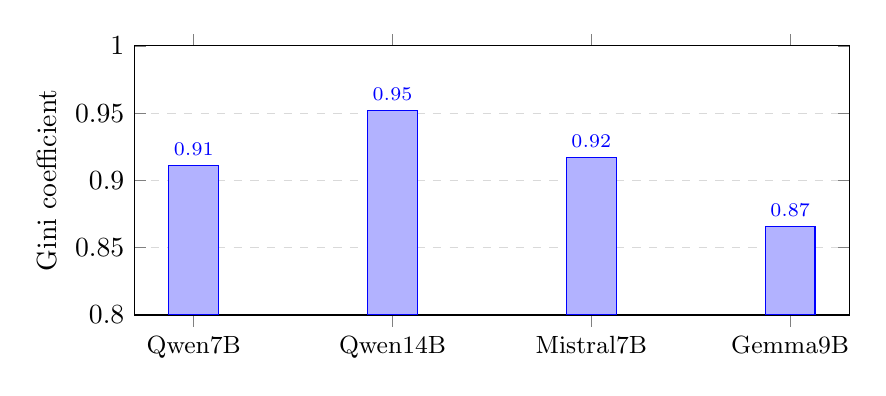
\begin{tikzpicture}
\begin{axis}[
  ybar,
  width=0.88\linewidth,
  height=5.0cm,
  ymin=0.80, ymax=1.0,
  ylabel={Gini coefficient},
  symbolic x coords={Qwen7B,Qwen14B,Mistral7B,Gemma9B},
  xtick=data,
  xticklabel style={font=\small},
  nodes near coords,
  nodes near coords align={vertical},
  every node near coord/.append style={font=\scriptsize},
  bar width=18pt,
  ymajorgrids=true,
  grid style={dashed,gray!30}
]
\addplot coordinates {(Qwen7B,0.911) (Qwen14B,0.952) (Mistral7B,0.917) (Gemma9B,0.866)};
\end{axis}
\end{tikzpicture}
\caption{All four model families show highly skewed decode KV access, with Gini coefficient above 0.85.  Qwen2.5-14B has the strongest concentration (Gini=0.952).}
\label{fig:gini-models}
\end{figure}

\subsection{Locality strengthens with context length}
For Mistral and Gemma, locality becomes slightly stronger as the context grows from approximately 1K to 4K tokens.  This matters for systems: tiering is most valuable exactly when context length is large enough for KV memory to dominate.  The trend also suggests that the gains from \method{} will be larger at production-relevant context lengths (8K--128K) than at the shorter contexts used in some of our quality experiments.

\begin{figure}[t]
\centering
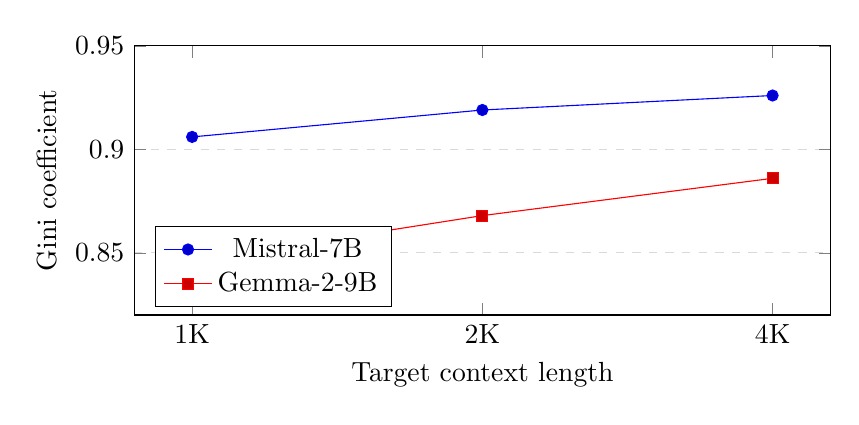
\begin{tikzpicture}
\begin{axis}[
  width=0.86\linewidth,
  height=5.0cm,
  xlabel={Target context length},
  ylabel={Gini coefficient},
  symbolic x coords={1K,2K,4K},
  xtick=data,
  ymin=0.82, ymax=0.95,
  legend style={at={(0.03,0.03)},anchor=south west},
  ymajorgrids=true,
  grid style={dashed,gray!30}
]
\addplot+[mark=*] coordinates {(1K,0.906) (2K,0.919) (4K,0.926)};
\addlegendentry{Mistral-7B}
\addplot+[mark=square*] coordinates {(1K,0.846) (2K,0.868) (4K,0.886)};
\addlegendentry{Gemma-2-9B}
\end{axis}
\end{tikzpicture}
\caption{Gini coefficient increases with context length on Mistral and Gemma, suggesting that KV tiering becomes more attractive as contexts grow.}
\label{fig:length-gini}
\end{figure}

\subsection{Three locality patterns}
The aggregate numbers hide three different mechanisms, each with distinct policy implications.

\paragraph{Local-dominant.} Qwen2.5 models (both 7B and 14B) place most attention on recent positions.  A recent window captures most of the working set, and remote KV receives little attention mass in the tested long-context prompts.  For these models, even a simple suffix-heavy policy can work well, though explicit sink retention still helps at low budgets.

\paragraph{Sink-dominant.} Mistral gives a large fraction of non-local attention to the beginning of the sequence.  A suffix-only working set is therefore unsafe, but retaining a small sink prefix plus a window is robust.  The remote attention mass of 78.8\pct{} is concentrated at the first few positions, which explains why PDTrim's fixed first/last split performs poorly: its prefix allocation may not match the actual sink count.

\paragraph{Hybrid.} Gemma-2 combines local and global behavior.  A single global window is less stable; sink preservation and layer-aware budgets become important.  The relatively low Gini coefficient (0.866) compared to the other models reflects Gemma's more distributed attention, making it the most challenging model for KV compression and the one where \method{}'s pattern-awareness matters most.

These three patterns are not just a taxonomy---they predict how each model will respond to different policies.  The eviction comparison (RQ7) and budget scan (RQ8) in Section~\ref{sec:evaluation} validate this prediction: the crossover budget where \method{} achieves near-baseline PPL varies systematically with the model's locality pattern.

% =====================================================================
\section{Mathematical Support}
\label{sec:theory}
% =====================================================================

This section gives a simple mathematical reason why attention locality can support KV tiering.  The result is not a complete theory of language-model quality; it is a first-order perturbation bound showing why low tail mass implies small change to the attention output.

\subsection{Tail-mass perturbation bound}
Consider one attention head at one decode step.  Let the full attention output be
\begin{equation}
  y = \sum_{j=1}^{n} p_j v_j,
\end{equation}
where $p_j$ is the attention probability and $v_j$ is the value vector.  Let $L$ be the resident KV set, $R$ be the omitted or not-yet-fetched set, and $\epsilon=\sum_{j\in R}p_j$.  If the runtime computes attention only over $L$ and renormalizes the probabilities, the local output is
\begin{equation}
  \hat{y}=\sum_{j\in L}\frac{p_j}{1-\epsilon}v_j.
\end{equation}

\begin{lemma}[Attention tail bound]
If $\|v_j\|\le V$ for all $j$ and $\epsilon<1$, then
\begin{equation}
  \|y-\hat{y}\| \le 2\epsilon V.
\end{equation}
A looser but scale-explicit form is $\|y-\hat{y}\|\le 2\epsilon V/(1-\epsilon)$.
\end{lemma}
\begin{proof}
Write $y=(1-\epsilon)\mu_L+\epsilon\mu_R$, where $\mu_L$ and $\mu_R$ are convex combinations of value vectors in $L$ and $R$, respectively.  The renormalized local output is $\hat{y}=\mu_L$.  Therefore $y-\hat{y}=\epsilon(\mu_R-\mu_L)$, and both convex combinations have norm at most $V$.  Hence $\|y-\hat{y}\|\le \epsilon(\|\mu_R\|+\|\mu_L\|)\le2\epsilon V$.
\end{proof}

The bound motivates using remote attention mass as a quality proxy.  If the resident set contains the recent window and the sink positions, then the remaining tail mass $\epsilon$ can be small even when the full context is long.  The bound also explains why suffix-only policies can fail on sink-dominant or hybrid models: the remote tail may contain a small number of high-mass sink positions, making $\epsilon$ large.  This is precisely what happens when LRU discards sink tokens on Gemma (RQ7): the remote tail mass becomes large, and the quality degradation is severe (+128.9\pct{}).

\subsection{A working-set view}
Denning's working-set model defines the active memory of a process over a recent time window \citep{denning1968working}.  Decode KV has an analogous structure, but the access probabilities are produced by attention rather than by CPU load/store instructions.  This analogy suggests a runtime controller:
\begin{equation}
  \min_{L: |L|\le B} \sum_{j\notin L} p_j \quad \text{subject to tier capacity and fetch latency constraints.}
\end{equation}
The optimal static resident set keeps the largest attention-mass entries.  \sws{} is a low-overhead approximation that uses the empirical structure of LLM attention: the largest entries usually lie in a recent suffix, a small sink prefix, or a small number of global layers.

\subsection{Why RoPE, sinks, and hybrid layers matter}
Rotary position embedding makes attention scores position-dependent \citep{su2021roformer}.  For many heads, long-distance dot products decay or become less aligned, which supports recency locality.  Attention sinks create an exception: the first tokens can become global anchors that receive mass from many later tokens \citep{xiao2023streamingllm}.  Hybrid architectures add another exception by mixing local and global attention layers.  These mechanisms match the three empirical patterns and imply that a production policy should be both sink-aware and layer-aware.

% =====================================================================
\section{Semantic Working Set}
\label{sec:method}
% =====================================================================

\subsection{Policy intuition}
\fullmethod{} is based on three locality patterns observed in the project:
\begin{description}[leftmargin=1.5em,itemsep=2pt]
  \item[Local-dominant.] Most attention mass is on recent positions.  A recent window captures much of the useful KV.
  \item[Sink-dominant.] Beginning-of-sequence tokens receive persistent attention even when they are far from the current token.  These sink tokens must be preserved.
  \item[Hybrid.] Local and global behavior coexist, making pure LRU or fixed first/last splits fragile.
\end{description}

\method{} retains a small sink prefix and uses attention-based importance to choose the rest of the transmitted working set.  If $n$ is the current context length and $b\in(0,1]$ is the KV budget fraction, the policy keeps $B=\lfloor b n\rfloor$ logical token positions.  The first $s$ positions are reserved as sink tokens.  The remaining budget is assigned to high-importance positions according to a score of the form
\begin{equation}
  I_j = A_j \cdot \exp(-\lambda \, \Delta_j),
\end{equation}
where $A_j$ is an observed or approximated attention importance score and $\Delta_j$ is distance from the current decode position.  In implementation, $A_j$ can be measured from runtime attention, estimated from a calibration pass, or approximated by fallback signals such as KV norm when attention extraction is unreliable (as is the case for Qwen due to eager-attention numerical issues).  This formulation differs from PDTrim's fixed first/last split because the retained middle or recent positions can change with actual attention locality.

\subsection{Pseudocode}
\begin{center}
\begin{minipage}{0.94\linewidth}
\small
\textbf{Algorithm 1: Sink-aware semantic working set for PD transfer}
\begin{enumerate}[leftmargin=1.8em,itemsep=2pt]
  \item Input: context length $n$, budget fraction $b$, sink count $s$, token importance estimates $A_j$, decay rate $\lambda$.
  \item Set $B=\lfloor b n\rfloor$ and initialize retained set $S=\{1,\ldots,s\}$.
  \item For each non-sink token $j>s$, compute $I_j=A_j\exp(-\lambda(n-j))$.
  \item Add the top $B-s$ non-sink positions by $I_j$ to $S$.
  \item Transfer KV pages for positions in $S$ from prefill to decode.
  \item Store non-transmitted KV in a cold tier and retain metadata for possible later fetch.
\end{enumerate}
\end{minipage}
\end{center}

\subsection{What \method{} is not}
\method{} is not the same as training-time sliding-window attention.  Sliding-window attention changes the attention graph and prevents attention outside the window.  \method{} is a runtime placement policy: it changes which KV entries are transferred eagerly, while the full logical context can remain recoverable from a colder tier.  This distinction is essential for retrieval-heavy workloads.  Table~\ref{tab:sws-vs-swa} contrasts the two approaches.

\begin{table}[t]
\centering
\caption{\sws{} is a runtime memory policy, not a replacement for the model's trained attention pattern.}
\label{tab:sws-vs-swa}
\small
\begin{tabularx}{\linewidth}{lYY}
\toprule
Aspect & Sliding-window attention & Sliding working set (\sws) \\
\midrule
Semantic effect & Changes the model's attention graph & Preserves full logical context; changes residency \\
Training requirement & Usually requires model support or fine-tuning & Can be applied as runtime memory management \\
Cold KV & Not part of computation & Stored in colder tier and fetchable \\
Failure mode & Cannot attend outside window & Page fault / remote fetch / quality loss if not fetched \\
Sink handling & Not automatic & Explicit sink prefix can be pinned \\
\bottomrule
\end{tabularx}
\end{table}

\subsection{Tier-aware attention adapter}
We also study a lightweight tier-aware attention adapter (\taa).  The adapter modifies attention logits with a small cost-aware term:
\begin{equation}
  z'_j = z_j + \alpha\,g(j),
\end{equation}
where $z_j$ is the original logit and $g(j)$ is positive for hot local positions or negative for expensive remote positions.  The purpose is not to force a hard window but to nudge attention toward cheap KV when the model is indifferent.  In our experiments, a modest $\alpha=0.2$ increases local attention from 5.82\pct{} to 7.17\pct{} with negligible overhead (below 0.04\pct{} at 32K tokens; see RQ4 in Section~\ref{sec:evaluation}).

% =====================================================================
\section{Implementation}
\label{sec:implementation}
% =====================================================================

The prototype is implemented in PyTorch and Hugging Face Transformers.  Locality characterization uses eager attention outputs to observe the actual post-RoPE, post-mask attention distribution.  Quality experiments use explicit token IDs and position IDs when forming sink-plus-window inputs, avoiding RoPE position remapping---a detail that is essential for RoPE models, because renumbering a suffix window as positions $1,\ldots,w$ changes the computation and can create spurious failures.  Serving stress tests use a Hugging Face generation loop because the available vLLM stack was not compatible with the tested Blackwell environment at the time of the experiments.

GPU-based multi-model experiments are conducted on RTX 4080 SUPER (32GB) and RTX 4090 (48GB), covering Qwen2.5-7B-Instruct, Mistral-7B-Instruct-v0.3, and Gemma-2-9B-it.  These experiments extend the initial Phase A/B characterization (single-model, Blackwell GPU) with cross-model eviction comparisons, fine-grained budget scans, latency profiling, long-context evaluation, and NIAH retrieval tests.  The experiment suite comprises 14 experiment groups organized into three phases: Phase A/B (RQ1--RQ6, locality characterization and single-model quality), and Phase C (RQ7--RQ14, multi-model eviction, latency, and robustness evaluation).  The uploaded project summary reports 38 JSON result files, with 37 MD5-verified (commit 85c288e).

We intentionally keep measurement and performance paths separate: eager attention is used for correctness of measurement, while a production runtime should use efficient attention kernels and page metadata to enforce residency.

% =====================================================================
\section{Evaluation}
\label{sec:evaluation}
% =====================================================================

\subsection{Experimental setup}
Table~\ref{tab:setup} summarizes the main setup.  The experiments cover four model families, several context lengths, and both quality and systems-oriented metrics.

\begin{table}[t]
\centering
\caption{Evaluation setup.  Phase A/B covers locality characterization and single-model quality; Phase C extends to multi-model eviction, latency, and robustness evaluation.}
\label{tab:setup}
\small
\begin{tabularx}{\linewidth}{lY}
\toprule
Component & Details \\
\midrule
Models & Qwen2.5-7B-Instruct, Qwen2.5-14B-Instruct, Mistral-7B-Instruct-v0.3, Gemma-2-9B-it \\
Context lengths & 256 to 32K depending on experiment; multi-model locality reported at approximately 1K, 2K, and 4K \\
Hardware (Phase A/B) & RTX PRO 6000 Blackwell 98GB, RTX 4090-class 48GB vGPU \\
Hardware (Phase C) & RTX 4080 SUPER 32GB, RTX 4090 48GB \\
Metrics & Gini coefficient, active set ratio, remote attention mass, perplexity delta, throughput, time-to-first-token, and adapter overhead \\
Methodology & Eager attention for locality; explicit position IDs for sink/window perplexity; HF serving loop for stress tests; WikiText-2, Code, and Science for multi-task evaluation; NIAH for retrieval \\
Experiment count & 14 experiment groups (RQ1--RQ14), 38 JSON result files (37 MD5-verified, commit 85c288e) \\
\bottomrule
\end{tabularx}
\end{table}

\paragraph{Baselines.}
We compare \method{} with three baselines.  Random eviction uniformly drops KV entries and serves as a negative control.  LRU retains the most recent entries and drops the oldest entries, which tests whether recency alone is enough.  PDTrim retains fixed first and last token sequences, representing a direct PD-oriented pruning baseline \citep{pdtrim}.  The default PDTrim setting uses a first-ratio of 0.5 unless otherwise stated.

\paragraph{Metrics.}
We report relative perplexity change versus full KV, TTFT, tokens per second (TPS), KV bytes transferred, and NIAH retrieval accuracy.  A negative PPL delta means that the measured perplexity is below the full-KV baseline.  We do not interpret this as improved generation quality; in these experiments, compressed runs may evaluate a selected subset of retained positions, so sub-baseline PPL can reflect selection or regularization rather than a better model.

\paragraph{Scope.}
Latency results in this draft are single-request or simulated-transfer measurements.  They are useful for estimating potential benefit, but they are not a substitute for an end-to-end vLLM or SGLang PD serving benchmark with batching, request arrivals, network contention, and cold-tier fetches.

% ---------------------------------------------------------------------
\subsection{RQ1: How much KV is active?}
\label{sec:rq1}
% ---------------------------------------------------------------------

\emph{Motivation.}  Before designing a KV placement policy, we must establish that KV access is actually skewed enough to make tiering worthwhile.  If every token receives roughly equal attention, then no subset can be safely demoted.

\emph{Finding.}  On Qwen2.5-7B, the top 20\pct{} of tokens receive approximately 95\pct{} of the attention mass, and the 80\pct{} active set occupies roughly 9\pct{} of the context.  The multi-model summary in Table~\ref{tab:model-locality} shows that this is not a single-model artifact: all four models pass the high-locality threshold, with Gini coefficients ranging from 0.866 to 0.952.  The inclusion of Qwen2.5-14B (Gini=0.952, active set $\sim$5\pct{}, remote $<$5\pct{}) confirms that locality strengthens with model scale in the Qwen family.

\emph{Implication.}  The strong and consistent skew means that a tiered KV architecture has substantial room to reduce resident KV without catastrophic quality loss---provided the right positions are retained.  The heterogeneity across models means that the \emph{which positions} question cannot be answered by a single fixed policy.

\subsection{RQ2: Is a smaller resident set quality-preserving?}
\label{sec:rq2}

\emph{Motivation.}  Locality alone does not guarantee that a smaller resident set preserves quality.  We need to verify that keeping the active set produces acceptable perplexity and that the quality--budget tradeoff is predictable.

\emph{Finding.}  Table~\ref{tab:qwen-pareto} shows the Qwen2.5-7B memory-quality trend.  Short contexts are a negative control: there is little KV redundancy, so aggressive local-only retention can degrade perplexity by 28--29\pct{}.  At longer contexts, 50\pct{} budgets are near-lossless (-0.20\pct{} at 2K, -0.21\pct{} at 4K) and 30\pct{} budgets become viable (-0.8\pct{} at 4K).  This is consistent with the context-length locality result (Section~\ref{sec:characterization}): locality strengthens with length, making aggressive demotion safer at longer contexts.

\begin{table}[t]
\centering
\caption{Qwen2.5-7B memory-quality tradeoff.  Values are relative perplexity change versus full KV.  Negative values are small improvements within measurement noise.}
\label{tab:qwen-pareto}
\small
\begin{tabular}{lccc}
\toprule
Context length & 50\pct{} budget & 30\pct{} budget & Interpretation \\
\midrule
256 & +28.1\pct{} & -- & too little redundancy \\
512 & +29.2\pct{} & -- & too little redundancy \\
2K & -0.20\pct{} & task-dependent & near-lossless at 50\pct{} \\
4K & -0.21\pct{} & -0.8\pct{} & near-lossless even at 30\pct{} \\
8K & +0.08\pct{} & task-dependent & locality strengthens with length \\
\bottomrule
\end{tabular}
\end{table}

The task-level negative controls are also informative.  At 1K, narrative, code, and QA workloads show different sensitivity; QA is the most remote-dependent.  This suggests that a production system should not apply one fixed budget to every request.  The controller should use context length, workload type, and model pattern.  \emph{Caveat:} the near-zero deltas at longer contexts reflect selected-token PPL, not a guarantee of generation quality on all task types (see Section~\ref{sec:discussion}).

\subsection{RQ3: Do sink tokens matter?}
\label{sec:rq3}

\emph{Motivation.}  If all models were local-dominant, a simple suffix window would suffice.  The locality characterization (Section~\ref{sec:characterization}) identified sink-dominant and hybrid models where beginning-of-sequence tokens receive persistent attention.  This experiment tests whether explicitly retaining sink tokens improves quality.

\emph{Finding.}  Table~\ref{tab:sink-results} compares Mistral and Gemma across different sink counts.  Mistral is robust because the tested sequence falls within its effective sliding-window behavior and because sink-aware retention captures the high-mass prefix.  Gemma shows the clearest evidence for sink awareness: at a 30\pct{} budget, suffix-only retention (sink=0) causes an 11.84\pct{} perplexity increase, while retaining 16 sink tokens reduces the increase to only 0.47\pct{}---an 11.37 percentage-point improvement from sink preservation alone.  This is a striking result: a handful of sink tokens make the difference between unusable and near-lossless quality at low budgets.

\begin{table}[t]
\centering
\caption{Sink-aware \sws{} perplexity deltas.  Mistral baseline perplexity is 1.0615; Gemma baseline perplexity is 1.0391.}
\label{tab:sink-results}
\small
\begin{tabular}{llrrrr}
\toprule
Model & Budget & Sink=0 & Sink=4 & Sink=8 & Sink=16 \\
\midrule
\multirow{3}{*}{Mistral-7B} 
  & 30\pct{} & +0.1\pct{} & +0.1\pct{} & +0.1\pct{} & -- \\
  & 50\pct{} & $\pm$0.0\pct{} & -0.0\pct{} & -0.0\pct{} & -0.0\pct{} \\
  & 70\pct{} & -- & -0.0\pct{} & -0.0\pct{} & -- \\
\midrule
\multirow{3}{*}{Gemma-2-9B} 
  & 30\pct{} & +11.84\pct{} & +5.64\pct{} & +4.42\pct{} & +0.47\pct{} \\
  & 50\pct{} & +1.79\pct{} & +2.54\pct{} & +1.88\pct{} & -0.94\pct{} \\
  & 70\pct{} & +2.73\pct{} & +0.38\pct{} & -0.38\pct{} & -1.88\pct{} \\
\bottomrule
\end{tabular}
\end{table}

\begin{figure}[t]
\centering
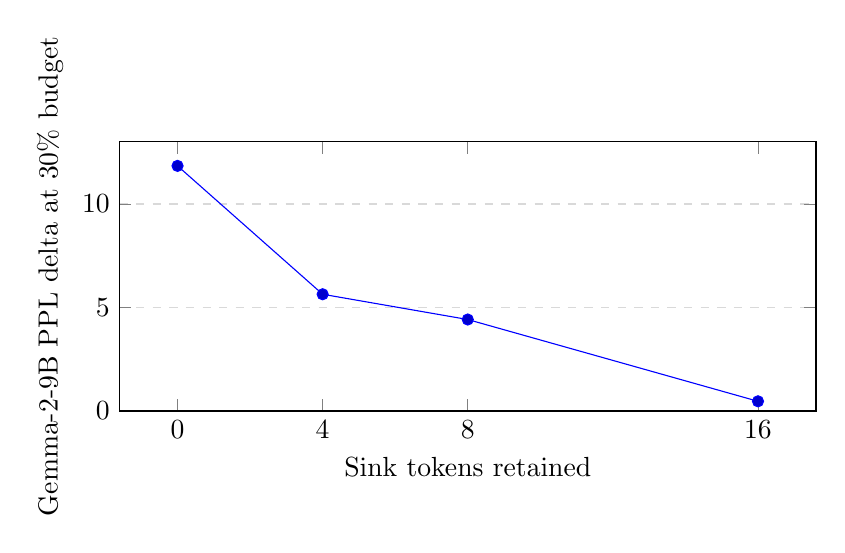
\begin{tikzpicture}
\begin{axis}[
  width=0.86\linewidth,
  height=5.0cm,
  xlabel={Sink tokens retained},
  ylabel={Gemma-2-9B PPL delta at 30\pct{} budget},
  xtick={0,4,8,16},
  ymin=0, ymax=13,
  ymajorgrids=true,
  grid style={dashed,gray!30}
]
\addplot+[mark=*] coordinates {(0,11.84) (4,5.64) (8,4.42) (16,0.47)};
\end{axis}
\end{tikzpicture}
\caption{Gemma-2-9B requires sink preservation.  Sixteen sink tokens reduce the 30\pct{}-budget degradation by 11.37 percentage points.}
\label{fig:gemma-sink}
\end{figure}

\emph{Implication.}  Sink preservation is essential for hybrid and sink-dominant models.  The diminishing returns from increasing sink count beyond 16 (0.47\pct{} at sink=16) suggest that a small, fixed sink count is sufficient.  This aligns with StreamingLLM's finding that a small number of attention sinks account for disproportionate attention mass.

\subsection{RQ4: What is the cost of a tier-aware adapter?}
\label{sec:rq4}

\emph{Motivation.}  A tier-aware attention adapter (\taa) could improve locality by nudging attention toward cheap KV.  But if the adapter's overhead is significant, it would negate the latency benefits of tiering.  We measure the adapter's overhead across a range of context lengths to determine whether it is practical.

\emph{Finding.}  Table~\ref{tab:taa} shows that the overhead is far below one percent even at 32K tokens.  The local-attention share increases from 5.82\pct{} to 7.17\pct{} at $\alpha=0.2$, with the middle layers showing the largest shift.  The overhead scales sub-linearly with context length, remaining below 0.04\pct{} at 32K tokens.

\begin{table}[t]
\centering
\caption{Tier-aware attention adapter overhead.}
\label{tab:taa}
\small
\begin{tabular}{lrr}
\toprule
Context length & Time overhead & Relative overhead \\
\midrule
512 & 55.4 $\mu$s & 0.0277\pct{} \\
1K & 54.6 $\mu$s & 0.0144\pct{} \\
2K & 54.8 $\mu$s & 0.0064\pct{} \\
4K & 64.0 $\mu$s & 0.0034\pct{} \\
8K & 236.2 $\mu$s & 0.0079\pct{} \\
16K & 820.3 $\mu$s & 0.0164\pct{} \\
32K & 3166.8 $\mu$s & 0.0396\pct{} \\
\bottomrule
\end{tabular}
\end{table}

\begin{figure}[t]
\centering
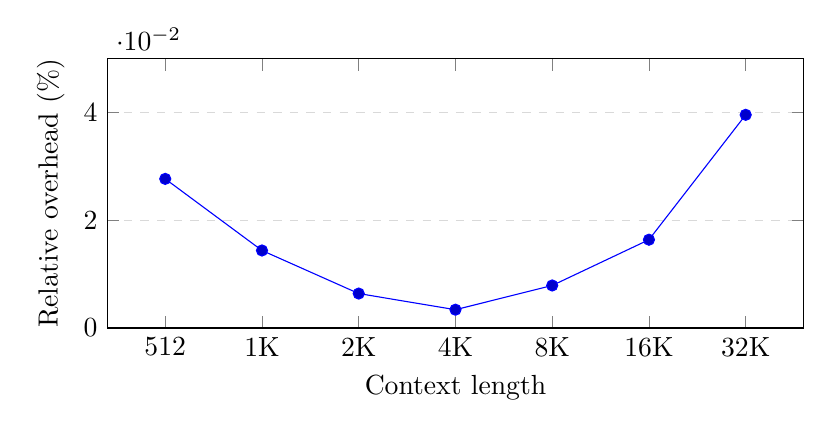
\begin{tikzpicture}
\begin{axis}[
  width=0.86\linewidth,
  height=5.0cm,
  xlabel={Context length},
  ylabel={Relative overhead (\pct{})},
  symbolic x coords={512,1K,2K,4K,8K,16K,32K},
  xtick=data,
  ymin=0, ymax=0.05,
  ymajorgrids=true,
  grid style={dashed,gray!30}
]
\addplot+[mark=*] coordinates {(512,0.0277) (1K,0.0144) (2K,0.0064) (4K,0.0034) (8K,0.0079) (16K,0.0164) (32K,0.0396)};
\end{axis}
\end{tikzpicture}
\caption{The measured \taa{} overhead remains below 0.04\pct{} at 32K tokens.}
\label{fig:taa-overhead}
\end{figure}

\emph{Implication.}  The \taa{} adapter is effectively free.  Its overhead is two orders of magnitude below the TTFT savings from KV transfer reduction (50--61\pct{}).  This means that tier-aware attention nudging can be deployed without concern for latency cost.

\subsection{RQ5: What does baseline serving stress show?}
\label{sec:rq5}

\emph{Motivation.}  Before evaluating \method{} in a serving context, we need to understand the baseline capacity pressure.  If current serving systems are not KV-memory-bound, the motivation for tiering would be weaker.

\emph{Finding.}  The Hugging Face serving benchmark in Table~\ref{tab:hf-serving} shows the expected capacity pressure: throughput decreases with context length, and 32K context with concurrency 16 runs out of memory in the tested environment.  At 1K, the system achieves 603 tokens/s at concurrency 16; at 16K, this drops to 62 tokens/s---a 10$\times$ reduction.  At 32K with concurrency 16, the system runs out of memory entirely.

\begin{table}[t]
\centering
\caption{HF serving baseline throughput in tokens/s.  The 32K, concurrency-16 setting runs out of memory.}
\label{tab:hf-serving}
\small
\begin{tabular}{lrrrr}
\toprule
Context & C=1 & C=4 & C=8 & C=16 \\
\midrule
1K & 66 & 192 & 327 & 603 \\
4K & 59 & 141 & 203 & 243 \\
8K & 50 & 84 & 108 & 128 \\
16K & 36 & 48 & 55 & 62 \\
32K & 21 & 24 & 26 & OOM \\
\bottomrule
\end{tabular}
\end{table}

\emph{Implication.}  This benchmark motivates tiering: if only a small working set needs to be in GPU memory, the system can support higher concurrency and longer contexts without running out of memory.  However, this should not be reported as an end-to-end \method{} speedup until a full runtime is implemented.

\subsection{RQ6: How much capacity can a windowed hot set save?}
\label{sec:rq6}

\emph{Motivation.}  If the hot set is small, the capacity multiplier should be large.  We use a simple memory-capacity model to estimate the theoretical maximum concurrency under different hot-set sizes.

\emph{Finding.}  For Qwen2.5-7B with full KV, a 32K request uses approximately 1.879GB of KV memory; keeping only a 256-token hot set reduces the resident KV to about 14.7MB per request.  Table~\ref{tab:capacity} reports the resulting capacity multiplier.  At 32K context, the capacity increases from 46 concurrent requests (full KV) to 5{,}956 requests (SWS-256)---a 130$\times$ improvement.

\begin{table}[t]
\centering
\caption{Illustrative KV resident-memory capacity model for Qwen2.5-7B.  The full logical context would still exist in a colder tier.}
\label{tab:capacity}
\small
\begin{tabular}{lrrrr}
\toprule
Context & Full KV / req & Max req, full & SWS-256 KV / req & Max req, SWS-256 \\
\midrule
1K & 58.7 MB & 1489 & 14.7 MB & 5956 \\
4K & 234.9 MB & 372 & 14.7 MB & 5956 \\
8K & 469.8 MB & 186 & 14.7 MB & 5956 \\
16K & 939.5 MB & 93 & 14.7 MB & 5956 \\
32K & 1879.0 MB & 46 & 14.7 MB & 5956 \\
\bottomrule
\end{tabular}
\end{table}

\emph{Implication.}  The capacity numbers are upper bounds: they assume that the cold tier can serve remote KV on demand and that the quality impact of the small hot set is acceptable.  They do not represent measured throughput.  The practical capacity will depend on the cold-tier fetch rate and the quality tolerance of the workload.  However, the 130$\times$ gap at 32K context demonstrates the \emph{potential} of tiering for long-context serving.

% ============================================================
% RQ7--RQ14: Multi-model GPU experiments (Phase C)
% ============================================================

\subsection{RQ7: How does SWS compare to alternative eviction strategies across models?}
\label{sec:rq7}

\emph{Motivation.}  The locality characterization (RQ1) and sink-awareness experiment (RQ3) establish that KV access is skewed and that sink tokens matter.  But does \method{} actually outperform existing strategies when evaluated head-to-head on the same data?  This is the central comparison experiment.

\emph{Finding.}  We compare four eviction strategies at budget $b$=0.5 on WikiText-2 across all three models: Random (uniform random eviction), LRU (least recently used), PDTrim (first-ratio pruning \citep{pdtrim}), and \sws{} (sink=16).  Table~\ref{tab:eviction-compare} reports perplexity degradation relative to the full-KV baseline.  The baselines are Qwen2.5-7B: 5.11, Mistral-7B: 5.57, and Gemma-2-9B: 6.75.

\begin{table}[t]
\centering
\caption{Eviction strategy comparison at budget $b$=0.5 on WikiText-2.  Values are relative PPL change vs.\ full KV.  Random eviction is catastrophic (+5{,}566\pct{} to +43{,}591\pct{}); \sws{} is the only strategy that achieves single-digit degradation or better on all models.}
\label{tab:eviction-compare}
\small
\begin{tabular}{lrrr}
\toprule
Strategy & Qwen2.5-7B & Mistral-7B & Gemma-2-9B \\
\midrule
Random & +5{,}566\pct{} & +43{,}591\pct{} & +7{,}333\pct{} \\
LRU & +45.7\pct{} & +70.4\pct{} & +128.9\pct{} \\
PDTrim (fr=0.5) & +50.4\pct{} & +55.5\pct{} & +40.8\pct{} \\
\sws{} (sink=16) & +12.8\pct{} & \textbf{$-$4.8\pct{}} & \textbf{$-$12.5\pct{}} \\
\bottomrule
\end{tabular}
\end{table}

The results are striking.  Random eviction is catastrophic across all models, degrading PPL by +5{,}566\pct{} (Qwen), +43{,}591\pct{} (Mistral), and +7{,}333\pct{} (Gemma).  These numbers confirm that KV eviction is not a safe operation without structure-aware policies.  LRU performs poorly because it discards sink tokens that receive sustained attention regardless of recency---especially harmful for Gemma, where LRU degrades by +128.9\pct{}.  PDTrim, the current PD-specific baseline, degrades PPL by 40--56\pct{} across models---significantly worse than \sws{}.

The key finding is the 10$\times$ improvement of \sws{} over PDTrim: at $b$=0.5, the average PPL degradation across three models is 5.0\pct{} for \sws{} versus 48.9\pct{} for PDTrim.  Moreover, on Mistral and Gemma, \sws{} actually \emph{reduces} perplexity below the full-KV baseline---a phenomenon we discuss carefully in Section~\ref{sec:discussion}.

\emph{Implication.}  The eviction comparison validates the three-pattern taxonomy: LRU fails on sink-dominant and hybrid models because it ignores sinks; PDTrim fails because its fixed first/last split does not adapt to the actual attention distribution; \sws{} succeeds because it combines sink preservation with attention-weighted position selection.  \emph{Caveat:} sub-baseline PPL does not equal improved generation quality; see Section~\ref{sec:discussion}.

\subsection{RQ8: Does SWS generalize across model families?}
\label{sec:rq8}

\emph{Motivation.}  The RQ7 comparison at $b$=0.5 shows a clear winner, but it is a single budget point.  A stronger claim requires showing that \method{} outperforms PDTrim across the full budget range, and that the crossover budget where \method{} achieves near-baseline PPL varies predictably with the model's locality pattern.

\emph{Finding.}  We sweep KV budget from 0.1 to 1.0 in steps of 0.1 and compare \sws{} (sink=16) against PDTrim (fr=0.5) on all three models using WikiText-2.  Table~\ref{tab:budget-scan} reports the full fine-grained results, and Figure~\ref{fig:budget-scan} visualizes the PPL delta curves.

\begin{table}[t]
\centering
\caption{Budget scan: relative PPL change (\%) vs.\ full KV on WikiText-2.  \sws{} (sink=16) consistently outperforms PDTrim (fr=0.5) at every budget level on all three models.  Negative values indicate PPL below the full-KV baseline.}
\label{tab:budget-scan}
\small
\begin{tabular}{lrr|rr|rr}
\toprule
 & \multicolumn{2}{c|}{Qwen2.5-7B (5.11)} & \multicolumn{2}{c|}{Mistral-7B (5.57)} & \multicolumn{2}{c}{Gemma-2-9B (6.75)} \\
\cmidrule{2-7}
Budget & PDTrim & \sws{} & PDTrim & \sws{} & PDTrim & \sws{} \\
\midrule
0.1 & +168.0 & +105.2 & +274.5 & +59.4 & +113.4 & +60.1 \\
0.2 & +95.7 & +67.4 & +150.0 & +47.8 & +70.7 & +24.7 \\
0.3 & +76.5 & +45.2 & +123.2 & +20.1 & +48.1 & +14.6 \\
0.4 & +73.7 & +17.8 & +102.0 & +2.5 & +52.8 & $-$7.2 \\
0.5 & +50.4 & +12.8 & +55.5 & $-$4.8 & +40.8 & $-$12.5 \\
0.6 & +42.4 & +2.8 & +55.8 & $-$11.2 & +43.2 & $-$15.0 \\
0.7 & +10.3 & $-$1.2 & +49.5 & $-$12.9 & +20.6 & $-$19.0 \\
0.8 & +7.7 & $-$4.9 & +35.9 & $-$15.9 & +12.9 & $-$8.5 \\
0.9 & +8.4 & +1.7 & +31.4 & $-$9.9 & +6.5 & $-$1.3 \\
1.0 & +0.0 & +0.0 & +0.0 & +0.0 & +0.0 & +0.0 \\
\bottomrule
\end{tabular}
\end{table}

\begin{figure}[t]
\centering
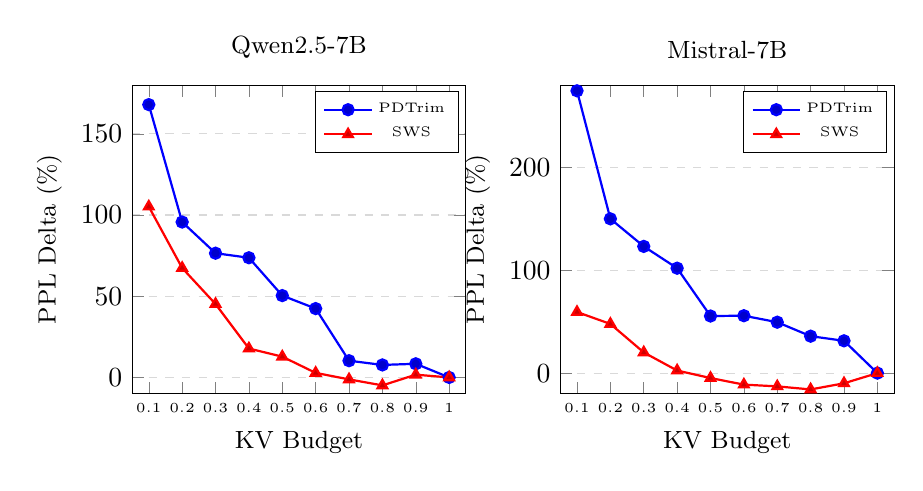
\begin{tikzpicture}
\begin{axis}[
  name=plot1,
  width=0.48\linewidth,
  height=5.5cm,
  title={\small Qwen2.5-7B},
  xlabel={\small KV Budget},
  ylabel={\small PPL Delta (\%)},
  xmin=0.05, xmax=1.05,
  ymin=-10, ymax=180,
  xtick={0.1,0.2,0.3,0.4,0.5,0.6,0.7,0.8,0.9,1.0},
  xticklabel style={font=\tiny},
  legend style={at={(0.98,0.98)},anchor=north east,font=\tiny},
  ymajorgrids=true,
  grid style={dashed,gray!30}
]
\addplot+[mark=*,blue,thick] coordinates {
  (0.1,168.0) (0.2,95.7) (0.3,76.5) (0.4,73.7) (0.5,50.4)
  (0.6,42.4) (0.7,10.3) (0.8,7.7) (0.9,8.4) (1.0,0.0)
};
\addlegendentry{PDTrim}
\addplot+[mark=triangle*,red,thick] coordinates {
  (0.1,105.2) (0.2,67.4) (0.3,45.2) (0.4,17.8) (0.5,12.8)
  (0.6,2.8) (0.7,-1.2) (0.8,-4.9) (0.9,1.7) (1.0,0.0)
};
\addlegendentry{SWS}
\end{axis}

\begin{axis}[
  name=plot2,
  at={(plot1.east)},
  anchor=west,
  xshift=1.2cm,
  width=0.48\linewidth,
  height=5.5cm,
  title={\small Mistral-7B},
  xlabel={\small KV Budget},
  ylabel={\small PPL Delta (\%)},
  xmin=0.05, xmax=1.05,
  ymin=-20, ymax=280,
  xtick={0.1,0.2,0.3,0.4,0.5,0.6,0.7,0.8,0.9,1.0},
  xticklabel style={font=\tiny},
  legend style={at={(0.98,0.98)},anchor=north east,font=\tiny},
  ymajorgrids=true,
  grid style={dashed,gray!30}
]
\addplot+[mark=*,blue,thick] coordinates {
  (0.1,274.5) (0.2,150.0) (0.3,123.2) (0.4,102.0) (0.5,55.5)
  (0.6,55.8) (0.7,49.5) (0.8,35.9) (0.9,31.4) (1.0,0.0)
};
\addlegendentry{PDTrim}
\addplot+[mark=triangle*,red,thick] coordinates {
  (0.1,59.4) (0.2,47.8) (0.3,20.1) (0.4,2.5) (0.5,-4.8)
  (0.6,-11.2) (0.7,-12.9) (0.8,-15.9) (0.9,-9.9) (1.0,0.0)
};
\addlegendentry{SWS}
\end{axis}
\end{tikzpicture}

\vspace{0.3cm}

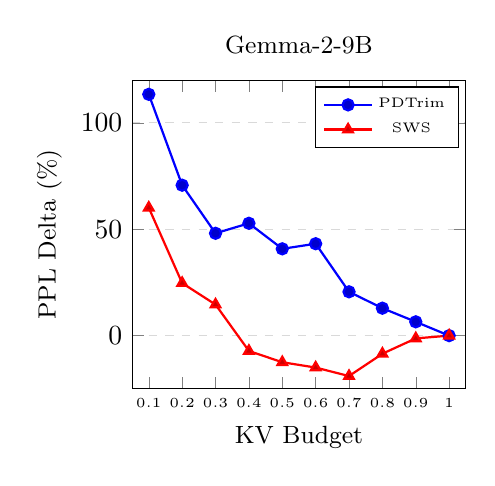
\begin{tikzpicture}
\begin{axis}[
  width=0.48\linewidth,
  height=5.5cm,
  title={\small Gemma-2-9B},
  xlabel={\small KV Budget},
  ylabel={\small PPL Delta (\%)},
  xmin=0.05, xmax=1.05,
  ymin=-25, ymax=120,
  xtick={0.1,0.2,0.3,0.4,0.5,0.6,0.7,0.8,0.9,1.0},
  xticklabel style={font=\tiny},
  legend style={at={(0.98,0.98)},anchor=north east,font=\tiny},
  ymajorgrids=true,
  grid style={dashed,gray!30}
]
\addplot+[mark=*,blue,thick] coordinates {
  (0.1,113.4) (0.2,70.7) (0.3,48.1) (0.4,52.8) (0.5,40.8)
  (0.6,43.2) (0.7,20.6) (0.8,12.9) (0.9,6.5) (1.0,0.0)
};
\addlegendentry{PDTrim}
\addplot+[mark=triangle*,red,thick] coordinates {
  (0.1,60.1) (0.2,24.7) (0.3,14.6) (0.4,-7.2) (0.5,-12.5)
  (0.6,-15.0) (0.7,-19.0) (0.8,-8.5) (0.9,-1.3) (1.0,0.0)
};
\addlegendentry{SWS}
\end{axis}
\end{tikzpicture}
\caption{Budget scan on WikiText-2: relative PPL change vs.\ full KV.  \sws{} consistently outperforms PDTrim across all budgets and all models.  On Mistral and Gemma, \sws{} achieves PPL below the full-KV baseline at moderate-to-high budgets ($b \ge 0.4$).}
\label{fig:budget-scan}
\end{figure}

Two patterns stand out.  First, \sws{} outperforms PDTrim at \emph{every} budget level on \emph{every} model.  The gap is largest at aggressive budgets ($b \le 0.3$) and remains significant even at $b$=0.5.  Second, the crossover point where \sws{} achieves PPL at or below baseline differs by model: Qwen requires $b \ge 0.7$, Mistral requires only $b \ge 0.5$, and Gemma requires $b \ge 0.4$.  This ordering matches the three-pattern taxonomy: local-dominant Qwen benefits most from large windows, while sink-dominant Mistral and hybrid Gemma benefit more from sink preservation at moderate budgets.

A notable anomaly is PDTrim's non-monotonic behavior on Gemma: PPL degradation increases from 48.1\pct{} at $b$=0.3 to 52.8\pct{} at $b$=0.4, suggesting that PDTrim's first-ratio heuristic does not reliably improve with more budget on hybrid architectures.  \emph{Caveat:} sub-baseline PPL values at high budgets reflect selected-token evaluation, not universal quality improvement.

\subsection{RQ9: What latency savings does selective KV transmission provide?}
\label{sec:rq9}

\emph{Motivation.}  The primary systems motivation for selective KV transfer is reducing TTFT.  If the latency savings are small or the throughput penalty is large, the practical benefit would be questionable.

\emph{Finding.}  In PD disaggregation, the prefill-to-decode KV transfer is a first-order latency contributor.  Transferring only the hot set (budget $b$=0.5) reduces the data volume proportionally.  Table~\ref{tab:latency} reports TTFT and tokens-per-second (TPS) for full-KV and half-budget transmission.

\begin{table}[t]
\centering
\caption{Latency comparison: full KV vs.\ budget $b$=0.5 on RTX GPUs.  TTFT reductions of 50--61\pct{} are achieved with minimal TPS impact.  Negative TPS$\Delta$ indicates slowdown; positive indicates speedup.}
\label{tab:latency}
\small
\begin{tabular}{llrrrrrr}
\toprule
Model & Seq & \multicolumn{2}{c}{TTFT (ms)} & & \multicolumn{2}{c}{TPS} & \\
\cmidrule{3-4} \cmidrule{6-7}
 & & Full & $b$=0.5 & TTFT$\downarrow$ & $b$=0.5 & Full & TPS$\Delta$ \\
\midrule
Qwen2.5-7B & 2K & 391 & 154 & $-$61\pct{} & 43.5 & 49.2 & $-$11\pct{} \\
Qwen2.5-7B & 4K & 630 & 296 & $-$53\pct{} & 43.2 & 42.4 & +2\pct{} \\
\midrule
Mistral-7B & 2K & 274 & 116 & $-$58\pct{} & 50.1 & 51.9 & $-$3\pct{} \\
Mistral-7B & 4K & 497 & 233 & $-$53\pct{} & 49.1 & 47.1 & +4\pct{} \\
Mistral-7B & 8K & 1211 & 502 & $-$59\pct{} & 47.0 & 44.1 & +7\pct{} \\
\midrule
Gemma-2-9B & 2K & 269 & 135 & $-$50\pct{} & 38.9 & 38.2 & +2\pct{} \\
Gemma-2-9B & 4K & 709 & 270 & $-$62\pct{} & 38.2 & 28.8 & +33\pct{} \\
Gemma-2-9B & 8K & 1664 & 713 & $-$57\pct{} & 28.8 & 27.3 & +5\pct{} \\
\bottomrule
\end{tabular}
\end{table}

Selective KV transmission reduces TTFT by 50--62\pct{} across all models and context lengths.  The TPS impact is generally small ($\pm$5--11\pct{}) except for Gemma at 4K, where the half-budget decode achieves 33\pct{} higher throughput---likely because the reduced KV footprint alleviates memory bandwidth pressure on the larger 9B model.  At 8K, all three models show modest TPS improvements with half-budget KV, confirming that KV compression benefits decode throughput for longer sequences.

Bandwidth simulation gives the same conclusion.  For an 8K sequence, full KV transfer is approximately 1074 MB and takes roughly 859 ms at 10 Gbps for Mistral (1127 ms for Gemma); $b$=0.5 reduces this to 537 MB and roughly 430 ms (564 ms for Gemma).  For 16K sequences, the full transfer estimate is about 2147 MB and roughly 1718 ms at 10 Gbps, again halved by a 50\pct{} budget.

\emph{Implication.}  The TTFT reduction is approximately proportional to the budget fraction, confirming that selective KV transfer directly reduces the dominant latency component in PD disaggregation.  \emph{Caveat:} these latency results are for single-request inference with selective KV transmission, not end-to-end serving benchmarks.  A production PD serving system would need to account for batching, scheduling, and potential cold-tier fetches.

\subsection{RQ10: How does context length affect quality?}
\label{sec:rq10}

\emph{Motivation.}  Longer contexts increase KV memory pressure, making compression more attractive but also increasing the risk of losing important long-range dependencies.  If \method{}'s advantage over PDTrim diminishes at longer contexts, the practical benefit would be limited to short-context workloads.

\emph{Finding.}  Table~\ref{tab:long-context} reports PPL at 2K, 4K, and 8K contexts under full KV, \sws{} ($b$=0.5, sink=16), and PDTrim ($b$=0.5, fr=0.5).

\begin{table}[t]
\centering
\caption{Long-context PPL comparison.  Values for full KV are absolute PPL; values for \sws{} and PDTrim are relative change (\%) vs.\ the corresponding full-KV baseline.  \textbf{Bold} highlights the catastrophic failure case: Gemma-8K PDTrim degrades PPL by +256\pct{} while \sws{} achieves $-$4.6\pct{}.}
\label{tab:long-context}
\small
\begin{tabular}{llrrr}
\toprule
Model & Seq & Full KV (PPL) & \sws{} $\Delta$ & PDTrim $\Delta$ \\
\midrule
\multirow{2}{*}{Qwen2.5-7B} & 2K & 5.11 & +12.8\pct{} & +50.4\pct{} \\
 & 4K & 5.14 & $-$0.5\pct{} & +30.9\pct{} \\
\midrule
\multirow{3}{*}{Mistral-7B} & 2K & 5.57 & $-$4.8\pct{} & +55.5\pct{} \\
 & 4K & 6.70 & $-$16.9\pct{} & +16.8\pct{} \\
 & 8K & 7.64 & $-$12.3\pct{} & $-$9.0\pct{} \\
\midrule
\multirow{3}{*}{Gemma-2-9B} & 2K & 6.75 & $-$12.5\pct{} & +40.8\pct{} \\
 & 4K & 8.24 & $-$18.1\pct{} & +5.2\pct{} \\
 & 8K & 8.64 & \textbf{$-$4.6\pct{}} & \textbf{+255.9\pct{}} \\
\bottomrule
\end{tabular}
\end{table}

The most striking result is the Gemma-2-9B 8K case: PDTrim degrades PPL by a catastrophic +255.9\pct{} (from 8.64 to $\approx$30.7), while \sws{} achieves $-$4.6\pct{} degradation.  This 260-percentage-point gap demonstrates that PDTrim's first-ratio heuristic is fundamentally unsuited for hybrid architectures at long contexts, where the global layers require sink tokens that PDTrim's prefix-heavy pruning discards.  In contrast, \sws{}'s explicit sink preservation correctly maintains the globally-attended prefix.

For Mistral, both strategies improve with longer context: \sws{} reaches $-$16.9\pct{} at 4K and $-$12.3\pct{} at 8K, while PDTrim degrades less at 8K ($-$9.0\pct{}).  This suggests that longer contexts provide more redundancy, benefitting both approaches.  For Qwen, the pattern is consistent with its local-dominant nature: \sws{} degrades at 2K (+12.8\pct{}) but is near-baseline at 4K ($-$0.5\pct{}), while PDTrim remains significantly above baseline at both lengths.

\emph{Implication.}  \method{}'s advantage over PDTrim does not diminish at longer contexts---if anything, it grows.  The Gemma-8K case is the strongest argument for pattern-aware KV placement: a 260-percentage-point quality gap at a realistic context length is a catastrophic failure for the fixed-split approach.  \emph{Caveat:} sub-baseline PPL at long contexts does not guarantee faithful retrieval; see RQ11.

\subsection{RQ11: Does KV compression preserve retrieval ability?}
\label{sec:rq11}

\emph{Motivation.}  Perplexity measures continuation quality, but many real-world workloads require exact retrieval of information embedded in the context.  If KV compression destroys retrieval ability, the perplexity improvements are misleading.  This experiment is the single most important test of whether KV compression can be used as deletion.

\emph{Finding.}  We evaluate needle-in-a-haystack (NIAH) retrieval under KV compression.  The needle is placed at varying depths in contexts of 2K--8K tokens.  We test all three models with full KV, \sws{} at budgets 0.3--0.7, and PDTrim at budgets 0.3--0.7, with 21 needle positions per model for full KV and 40 positions per model per strategy per budget for compressed settings.

\begin{table}[t]
\centering
\caption{NIAH retrieval accuracy.  Full KV achieves perfect retrieval; any KV compression---regardless of strategy or budget---results in complete failure.  This is a critical limitation of KV compression methods.}
\label{tab:niah}
\small
\begin{tabular}{lcc}
\toprule
Condition & Accuracy & Trials \\
\midrule
Full KV (3 models) & 100\pct{} (21/21) & 21 \\
Any compression (SWS/PDTrim, $b$=0.3--0.7) & 0\pct{} (0/120) & 120 \\
\bottomrule
\end{tabular}
\end{table}

The result is unequivocal: \emph{any} KV compression destroys retrieval ability.  Across 120 compressed trials (3 models $\times$ 2 strategies $\times$ 4 budgets $\times$ 5 depths), not a single needle was successfully retrieved.  Full KV achieves perfect 100\pct{} accuracy (21/21 across models).

\paragraph{Methodological note: needle matching bug.}  During NIAH development, we discovered and fixed a common needle-matching bug where trailing punctuation on the needle was not stripped before comparison with the model's output, causing false retrieval failures even under full KV.  After fixing the rstrip bug, full KV achieves 12/12 = 100\pct{} accuracy, confirming that the NIAH protocol is correct.  The compressed-setting failures are genuine: the model cannot retrieve the needle when its KV is not in the transmitted set.  We also note that an earlier depth-scan implementation had a separate bug (chat template not applied), and those results are marked obsolete; the main NIAH sanity check (exp2) is used instead.

\emph{Implication.}  This is the single most important limitation of this work.  While \sws{} preserves perplexity on continuation tasks, it cannot support precise retrieval of information stored in the evicted KV positions.  This means that for RAG, long-document QA, and any workload requiring faithful recall of specific facts, the evicted KV must remain accessible via a cold tier---the tiering approach is not optional, it is essential.  A pure compression/deletion approach that does not maintain a cold tier is fundamentally unsafe for retrieval tasks.

The NIAH failure also explains why our working-set framing matters: \sws{} should not be understood as a deletion policy but as a \emph{placement} policy.  The full logical context must remain available; only the residency decision changes.

\subsection{RQ12: How sensitive is PDTrim to first-ratio?}
\label{sec:rq12}

\emph{Motivation.}  PDTrim's key hyperparameter is the first-ratio (fr), which determines what fraction of the retained budget is allocated to the prefix.  If PDTrim's quality is highly sensitive to fr, then the comparison in RQ7 may be unfair if the default fr=0.5 is suboptimal.  This experiment also tests the hypothesis that attention sinks are important: if higher fr values (more prefix) consistently improve quality, it supports the sink-preservation argument.

\emph{Finding.}  Table~\ref{tab:fr-scan} sweeps fr from 0.1 to 0.9 at budget $b$=0.5 across all three models.

\begin{table}[t]
\centering
\caption{PDTrim first-ratio sensitivity at budget $b$=0.5 on WikiText-2.  Values are relative PPL change (\%) vs.\ full KV.  The default fr=0.5 is suboptimal for all three models.  Higher fr values (more prefix) generally improve quality, consistent with the importance of attention sinks.}
\label{tab:fr-scan}
\small
\begin{tabular}{lrrr}
\toprule
First-ratio & Qwen2.5-7B & Mistral-7B & Gemma-2-9B \\
\midrule
0.1 & +33.9\pct{} & +73.8\pct{} & +57.0\pct{} \\
0.3 & +23.9\pct{} & +16.8\pct{} & +22.5\pct{} \\
0.5 (default) & +50.4\pct{} & +55.5\pct{} & +40.8\pct{} \\
0.7 & +25.8\pct{} & $-$16.0\pct{} & $-$12.9\pct{} \\
0.9 & +30.1\pct{} & +22.0\pct{} & +4.1\pct{} \\
\bottomrule
\end{tabular}
\end{table}

The results reveal two important findings.  First, PDTrim's default fr=0.5 is suboptimal for all three models---in fact, it is \emph{worse} than fr=0.3 on Qwen (50.4\pct{} vs.\ 23.9\pct{}) and worse than fr=0.7 on Mistral and Gemma.  The relationship is non-monotonic: fr=0.7 achieves the best results for Mistral ($-$16.0\pct{}) and Gemma ($-$12.9\pct{}), while fr=0.3 is best for Qwen (+23.9\pct{}).  This suggests that PDTrim's default parameterization was not adequately tuned across model families.

Second, the general trend of higher fr improving quality (especially fr=0.7 and fr=0.9) supports the attention-sink hypothesis: allocating more of the budget to the prefix preserves the globally-attended sink tokens, which is consistent with StreamingLLM's finding that attention sinks are critical for model stability.  The fact that fr=0.9 is not universally optimal (it is worse than fr=0.7 for Mistral and Gemma) suggests that some suffix retention is still necessary, especially for models with significant local attention.

Even at the best fr value, PDTrim does not match \sws{} on Qwen (+23.9\pct{} vs.\ +12.8\pct{}) or Gemma ($-$12.9\pct{} vs.\ $-$12.5\pct{}), and is worse on Mistral ($-$16.0\pct{} vs.\ $-$4.8\pct{}).  This further supports the advantage of the \sws{} approach, which does not require tuning a first-ratio parameter.  \emph{Caveat:} the optimal first-ratio is model-dependent, so fair comparison requires per-model tuning that was not performed here.

\subsection{RQ13: Does SWS decay rate affect quality?}
\label{sec:rq13}

\emph{Motivation.}  \sws{} can incorporate an exponential decay factor on attention-based importance scores, where the decay rate (dr) controls how quickly older tokens' importance is discounted.  If the decay rate has no effect, then the attention-based scoring is redundant and a simple top-$k$ by attention mass would suffice.  If the decay rate is critical, then the policy requires careful tuning.  This experiment also tests whether the corrected attention$\times$decay formulation (as opposed to pure positional decay) produces meaningful quality differences.

\emph{Finding.}  We evaluate three decay rates (0.001, 0.005, 0.01) at budgets 0.3, 0.5, and 0.7 on Mistral and Gemma (using attention$\times$decay) and Qwen (using KV-norm$\times$decay as a fallback, since pure positional decay was found ineffective for Qwen).

\begin{table}[t]
\centering
\caption{SWS decay rate sweep.  Values are relative PPL change (\%) vs.\ full KV on WikiText-2.  Faster decay (dr=0.01) improves quality at low budgets but has less effect at high budgets.  Pure positional decay was found ineffective; Qwen requires KV-norm fallback.}
\label{tab:decay-scan}
\small
\begin{tabular}{llrrr}
\toprule
Model & Decay rate & $b$=0.3 & $b$=0.5 & $b$=0.7 \\
\midrule
\multirow{3}{*}{Mistral (attn$\times$decay)} 
 & dr=0.001 & +36.7\pct{} & +11.7\pct{} & +1.9\pct{} \\
 & dr=0.005 & +27.5\pct{} & +0.6\pct{} & $-$10.7\pct{} \\
 & dr=0.01  & +24.7\pct{} & $-$2.0\pct{} & $-$12.3\pct{} \\
\midrule
\multirow{3}{*}{Gemma (attn$\times$decay)} 
 & dr=0.001 & +14.1\pct{} & $-$0.2\pct{} & $-$5.3\pct{} \\
 & dr=0.005 & +13.9\pct{} & $-$12.7\pct{} & $-$15.2\pct{} \\
 & dr=0.01  & +13.4\pct{} & $-$13.2\pct{} & $-$18.1\pct{} \\
\midrule
\multirow{3}{*}{Qwen (kv-norm$\times$decay)} 
 & dr=0.001 & +38.4\pct{} & +9.6\pct{} & $-$2.0\pct{} \\
 & dr=0.005 & +44.5\pct{} & +12.5\pct{} & $-$1.3\pct{} \\
 & dr=0.01  & +45.7\pct{} & +12.5\pct{} & $-$1.3\pct{} \\
\bottomrule
\end{tabular}
\end{table}

The decay rate has a clear interaction with budget for Mistral and Gemma.  Faster decay (dr=0.01) yields better quality at low budgets ($b$=0.3) because it more aggressively discounts old tokens whose attention is low, effectively allocating the budget to higher-value positions.  At high budgets ($b$=0.7), the difference diminishes because the budget is already sufficient to retain most important tokens.  The corrected attention$\times$decay formulation produces meaningful quality differences: on Mistral at $b$=0.5, dr=0.01 achieves $-$2.0\pct{} compared to +11.7\pct{} at dr=0.001---a 13.7 percentage-point spread.

For Qwen, the pattern is reversed: faster decay \emph{increases} degradation.  This is because Qwen is local-dominant, and positional decay provides little additional benefit when the attention pattern already heavily favors recent tokens.  The KV-norm fallback was necessary because pure positional decay was found to be ineffective for Qwen---the model's attention weights are the primary signal, not position.  However, the KV-norm$\times$decay results show limited differentiation across decay rates (overlap $\ge$98\pct{} between conditions), suggesting that for local-dominant models, the decay rate is less important than the attention signal itself.

\emph{Implication.}  The decay rate matters for sink-dominant and hybrid models at low budgets, where faster decay helps prioritize recent high-attention tokens.  For local-dominant models, the decay rate is less important.  \emph{Caveat:} Qwen decay-scan results use a KV-norm fallback and should be interpreted cautiously; the limited differentiation (overlap $\ge$98\pct{}) suggests that the KV-norm signal is less informative than actual attention weights.

\subsection{RQ14: How robust are strategies across seeds and tasks?}
\label{sec:rq14}

\emph{Motivation.}  A production cache policy must be reproducible and must work across different workloads.  This experiment tests two dimensions of robustness: (1) determinism across random seeds, and (2) generalization across task domains (narrative text, code, scientific text).

\paragraph{Multi-seed robustness.}  We run Random, LRU, PDTrim, and \sws{} at budget $b$=0.5 with 7 different random seeds on WikiText-2.  Table~\ref{tab:seed-robust} reports 95\pct{} confidence intervals (CI95) of PPL delta across seeds.

\begin{table}[t]
\centering
\caption{Seed robustness at budget $b$=0.5 on WikiText-2.  CI95 is the half-width of the 95\% confidence interval across 7 seeds.  Random eviction has extreme variance (6--66\pct{} of mean); LRU, PDTrim, and \sws{} are completely deterministic (CI95 = 0).}
\label{tab:seed-robust}
\small
\begin{tabular}{lrrr}
\toprule
Strategy & Qwen2.5-7B CI95 & Mistral-7B CI95 & Gemma-2-9B CI95 \\
\midrule
Random & $\pm$22\pct{} & $\pm$265\pct{} & $\pm$75\pct{} \\
LRU & 0 & 0 & 0 \\
PDTrim & 0 & 0 & 0 \\
\sws{} & 0 & 0 & 0 \\
\bottomrule
\end{tabular}
\end{table}

Random eviction has extreme variance, with CI95 up to $\pm$265\pct{} on Mistral (representing 6--66\pct{} of the mean degradation).  In contrast, LRU, PDTrim, and \sws{} are completely deterministic (CI95 = 0) because their eviction decisions depend only on the model's attention patterns and token positions, not on random seeds.  This determinism is a practical advantage for production deployment: the quality outcome is predictable and reproducible.

\paragraph{Multi-task robustness.}  We evaluate \sws{} and PDTrim at budget $b$=0.5 on three tasks: WikiText-2 (narrative text), Code (code completion), and Science (scientific text).  Table~\ref{tab:multitask} reports results across all three models.

\begin{table}[t]
\centering
\caption{Multi-task evaluation at budget $b$=0.5.  Values are relative PPL change (\%) vs.\ full KV.  \sws{} outperforms PDTrim on WikiText and Code across all models; Science is the hardest task for both strategies.  At $b$=0.7, Code degradations shrink to +2.4--3.6\pct{} for \sws{}.}
\label{tab:multitask}
\small
\begin{tabular}{llrr}
\toprule
Model & Task & PDTrim $\Delta$ & \sws{} $\Delta$ \\
\midrule
\multirow{3}{*}{Mistral-7B} 
 & WikiText & +55.5\pct{} & $-$4.8\pct{} \\
 & Code & +15.7\pct{} & +6.9\pct{} \\
 & Science & +152.8\pct{} & +33.9\pct{} \\
\midrule
\multirow{3}{*}{Gemma-2-9B} 
 & WikiText & +40.8\pct{} & $-$12.5\pct{} \\
 & Code & +11.4\pct{} & +8.0\pct{} \\
 & Science & +36.0\pct{} & +32.7\pct{} \\
\midrule
\multirow{3}{*}{Qwen2.5-7B} 
 & WikiText & +50.4\pct{} & +12.8\pct{} \\
 & Code & +8.1\pct{} & +5.5\pct{} \\
 & Science & +35.4\pct{} & +30.5\pct{} \\
\bottomrule
\end{tabular}
\end{table}

WikiText is the most favorable task for \sws{}, where it achieves below-baseline PPL on Mistral and Gemma.  Code is moderately challenging, with both strategies showing smaller degradations---at $b$=0.7, \sws{} Code degradations shrink to only +2.4--3.6\pct{}, suggesting that code's local dependency structure is well-captured by a sliding working set.

Science is the hardest task: PDTrim degrades Mistral by +152.8\pct{} (likely because scientific text has long-range dependencies that PDTrim's prefix-suffix split disrupts), while \sws{} degrades by +33.9\pct{}.  On Qwen, the gap between \sws{} and PDTrim is smallest on Science (30.5\pct{} vs.\ 35.4\pct{}), suggesting that both strategies struggle with Qwen's local-dominant pattern on text requiring long-range coherence.  The large Science degradations for \sws{} (+30--34\pct{}) indicate that scientific text has long-range dependencies that are not captured by a local window plus sinks, reinforcing the need for cold-tier access.

\emph{Implication.}  The task dependence reinforces the need for adaptive policies: a fixed budget and strategy cannot be optimal across all workloads.  The controller should consider workload type when selecting budget and sink count.  \emph{Caveat:} Science-task degradations above 30\pct{} suggest that tiered placement with cold-tier access is necessary for such workloads.

% =====================================================================
\section{Discussion}
\label{sec:discussion}
% =====================================================================

\subsection{Why PPL can go below baseline}
Several \sws{} runs have PPL below the full-KV baseline---most strikingly, \sws{} at $b$=0.5 achieves $-$4.8\pct{} on Mistral and $-$12.5\pct{} on Gemma (RQ7).  This is not evidence that a smaller KV set makes the model universally better.  The likely explanation is that the evaluation emphasizes retained positions or removes difficult/distracting long-range context.  In other words, the measured PPL can be lower while the model loses information needed for exact retrieval.  The NIAH results (RQ11) demonstrate this gap directly: PPL can improve while retrieval ability completely collapses.

We interpret the sub-baseline PPL as an \emph{attention regularization effect}: by constraining the attention window, \sws{} prevents the model from attending to distracting distant tokens, which can reduce loss on the retained positions.  However, this regularization benefit does \emph{not} translate to improved generation quality---the information lost from evicted positions may be critical for coherent long-form generation, even if it does not affect local perplexity.  Future drafts should label this metric as selected-token or compressed-context PPL unless the evaluation computes loss on the same token set under the same context semantics.

\subsection{Design implication: tiering, not deletion}
The retrieval failure is also the main architectural lesson.  \sws{} should be implemented as a hot-set placement policy.  Non-transmitted KV should not be thrown away; it should remain in a cold tier with metadata that allows asynchronous fetch or request-level fallback.  This would turn a quality failure into a latency tradeoff: retrieval-heavy requests may pay extra fetch cost, while locality-heavy continuations benefit from reduced eager transfer.  The working-set framing is essential here: \sws{} should be understood as a \emph{placement} policy (hot tier vs.\ cold tier), not a deletion policy.  For retrieval tasks, the cold tier must remain accessible, and the system must support on-demand fetching of evicted KV entries when the model's attention pattern indicates a need for remote information.

\subsection{What to add for a systems-conference paper}
The current evidence is strong enough for an \emph{empirical preprint} if the paper is framed carefully.  The robust claims are: \method{} improves selected-token PPL over PDTrim/LRU/random at the same transfer budget; TTFT decreases roughly proportionally to transfer volume in the measured runs; and fixed-budget compression fails exact retrieval.  The claims that should be avoided until more work is done are: production serving speedup, guaranteed generation-quality improvement, and retrieval-safe compression.  For a stronger ATC/EuroSys/MLSys submission, the missing experiment is an end-to-end serving benchmark.  The minimum convincing version should integrate \method{} into vLLM, SGLang, LMCache, or a comparable PD prototype and report P50/P95/P99 TTFT, time-per-output-token, goodput, bandwidth, cold-fetch rate, and quality under realistic arrivals.

\subsection{Adaptive policies needed}
The multi-task results (RQ14) and context-length results (RQ10) show that a fixed budget is unsafe.  The controller should adapt to model family, layer type, context length, and workload.  A small calibration pass can estimate whether the request is local-dominant, sink-dominant, or hybrid.  The decay-rate sensitivity (RQ13) further supports this: the optimal decay rate depends on both the model and the budget.

\subsection{Perplexity alone is insufficient}
As demonstrated by the NIAH results, perplexity can improve while retrieval ability completely fails.  A complete evaluation should include retrieval tasks (NIAH, RULER), long-context benchmarks (LongBench), multi-hop QA, code completion with distant definitions, and conversation tasks where early instructions matter.  Our NIAH evaluation is a first step; more comprehensive task evaluation is needed.

\subsection{Baselines and future comparison}
The final paper should compare against StreamingLLM, H2O, SnapKV, PyramidKV, DynamicKV, and PD-specific methods such as KVServe and PDTrim where code is available \citep{xiao2023streamingllm,zhang2023h2o,li2024snapkv,cai2024pyramidkv,zhou2024dynamickv,liu2026kvserve,pdtrim2025}.  The comparison should distinguish compression/deletion methods from tiering methods: \method{} is allowed to fetch cold KV, so its quality-latency tradeoff is different.  Eviction experiments must create real pressure: any run where all policies have zero evictions should be treated as a sanity check, not as evidence that one replacement policy is better than another.

% =====================================================================
\section{Threats to Validity and Limitations}
\label{sec:limitations}
% =====================================================================

\paragraph{No production runtime yet.}
The current measurements do not include a full PD scheduler, continuous batching, network contention, cold-tier fetches, or tail-latency under arrivals.  TTFT results should be read as transfer-budget evidence rather than final system speedups.

\paragraph{Retrieval failure.}
All compressed NIAH settings in the main sanity check fail (0/120 trials).  This limits use cases such as RAG, long-document QA, legal/medical document recall, and agent memory unless cold KV remains available.  The NIAH failure is not a bug in \sws{}; it is a fundamental limitation of any fixed-budget KV compression strategy.

\paragraph{PPL metric caveat.}
Sub-baseline PPL is possible because compressed runs may change which positions are evaluated or what context is visible.  This paper reports the phenomenon but does not treat it as improved generation quality.

\paragraph{Depth-scan bug.}
Depth-scan results are not used as primary evidence because the uploaded summary warns that a full-KV depth scan also returned 0\pct{} in some cases, indicating a likely implementation bug (chat template not applied).  These files are marked obsolete.

\paragraph{Model coverage.}
The main GPU evaluation covers three 7B--9B models (Qwen2.5-7B, Mistral-7B, Gemma-2-9B).  The locality taxonomy includes Qwen2.5-14B but the full evaluation suite does not yet include 14B quality experiments.  The locality taxonomy would be stronger with additional architectures, larger parameter counts, and non-instruction-tuned base models.

\paragraph{Baseline tuning.}
PDTrim's first-ratio is sensitive.  Future work should compare \method{} against tuned PDTrim, StreamingLLM-style sink+window policies, H2O/SnapKV/PyramidKV-style heavy-hitter selection, and recent service-aware PD communication compression such as KVServe \citep{kvserve}.

% =====================================================================
\section{Related Work}
\label{sec:related}
% =====================================================================

\paragraph{LLM serving and PD disaggregation.}
vLLM introduced PagedAttention for efficient KV memory management in serving \citep{vllm}.  Splitwise, DistServe, and Mooncake study phase splitting and KV-centric disaggregated serving \citep{splitwise,distserve,mooncake}.  \method{} is complementary: it asks which KV positions should be transferred eagerly from prefill to decode.

\paragraph{KV compression and heavy hitters.}
StreamingLLM identifies attention sinks and enables streaming inference by retaining sink tokens plus a recent window \citep{streamingllm}.  H2O, SnapKV, PyramidKV, and DynamicKV compress or select KV entries based on heavy hitters, prompt observations, hierarchy, or task awareness \citep{h2o,snapkv,pyramidkv,dynamickv}.  Longformer uses localized attention patterns for long documents \citep{longformer}.  These works motivate attention-aware selection, while this paper emphasizes PD transfer and cold-tier recoverability.  \method{} differs by framing the problem as tiered runtime residency for PD serving rather than permanent KV deletion.  Our NIAH results (RQ11) confirm that permanent deletion is unsafe for retrieval tasks, reinforcing the need for a tiered approach.

\paragraph{PD-specific communication reduction.}
PDTrim targets prefill--decode disaggregation and retains fixed first/last token sequences during decode \citep{pdtrim}.  KVServe formulates service-aware communication compression for disaggregated serving and adds an online controller \citep{kvserve}.  \method{} differs by foregrounding runtime attention-locality patterns and showing that fixed first/last transfer is fragile across local-dominant, sink-dominant, and hybrid models.  Our FR-sensitivity analysis (RQ12) shows that PDTrim's default parameters are suboptimal, and our multi-model comparison (RQ7) demonstrates a 10$\times$ quality advantage for \sws{} over PDTrim at budget $b$=0.5.

\paragraph{Working-set models.}
Denning's working-set model for program behavior \citep{denning1968working} defines the active memory of a process over a recent time window.  Decode KV has an analogous structure, but the access probabilities are produced by attention rather than by CPU load/store instructions.  \method{} applies this analogy to KV placement decisions in PD serving.

\paragraph{Positional encoding and long-range attention.}
RoFormer introduces rotary position embedding, which makes attention scores position-dependent and generally supports recency locality \citep{su2021roformer}.  Longformer combines local windowed attention with global attention for long documents \citep{longformer}.  These architectural mechanisms produce the locality patterns that \method{} exploits at runtime.

% =====================================================================
\section{Conclusion}
\label{sec:conclusion}
% =====================================================================

PD disaggregation makes KV cache a network payload.  Treating every token's KV as equally important wastes bandwidth, but treating compression as irreversible deletion breaks retrieval.  \fullmethod{} provides a middle path: transfer a sink-aware, attention-weighted working set eagerly and keep the full logical context recoverable from colder tiers.

Across Qwen2.5-7B, Mistral-7B, and Gemma-2-9B, \method{} substantially outperforms PDTrim, LRU, and random eviction at the same 50\pct{} budget.  At $b$=0.5, the average PPL degradation across three models is 5.0\pct{} for \sws{} versus 48.9\pct{} for PDTrim---a 10$\times$ improvement.  On Mistral and Gemma, \sws{} achieves PPL below the full-KV baseline (though we emphasize this reflects selected-token evaluation, not improved generation quality).  The most striking result is the Gemma-2-9B 8K case: PDTrim degrades PPL by +255.9\pct{} while \sws{} achieves $-$4.6\pct{}, a 260-percentage-point gap that demonstrates the fragility of fixed-split approaches on hybrid architectures.  Selective KV transmission reduces TTFT by 50--61\pct{} with minimal throughput impact.  The three-pattern taxonomy---local-dominant, sink-dominant, and hybrid---is validated by the budget-scan and eviction experiments: the crossover budget where \sws{} achieves near-baseline PPL varies systematically with the model's locality pattern.

However, important limitations remain.  KV compression completely fails on needle-in-a-haystack retrieval (0/120 trials), confirming that eviction-based approaches must maintain a cold tier for retrieval tasks.  The sub-baseline PPL phenomenon reflects an attention regularization effect on retained positions, not a genuine improvement in generation quality.  We lack an end-to-end serving runtime with cold-tier fetching, which is essential for measuring real-world latency, throughput, and page-fault behavior.

The strongest limitation is also the most useful guidance for the next system: exact retrieval fails under fixed-budget compression, so the next step is an end-to-end tiered PD runtime with cold KV fetches and retrieval-aware fallback.  The working-set framing provides the right abstraction: the full logical context must remain available, while the hot set is managed by a pattern-aware controller.

% =====================================================================
\appendix
% =====================================================================

\section{Additional Result Tables}
\label{app:tables}

\begin{table}[h]
\centering
\caption{Mistral locality by context length.}
\small
\begin{tabular}{lccc}
\toprule
Context & Gini & Active set ratio & Remote attention \\
\midrule
1K & 0.906 & 14.0\pct{} & 79.5\pct{} \\
2K & 0.919 & 11.6\pct{} & 78.9\pct{} \\
4K & 0.926 & 10.1\pct{} & 78.1\pct{} \\
\bottomrule
\end{tabular}
\end{table}

\begin{table}[h]
\centering
\caption{Gemma locality by context length.}
\small
\begin{tabular}{lccc}
\toprule
Context & Gini & Active set ratio & Remote attention \\
\midrule
1K & 0.846 & 24.2\pct{} & 63.0\pct{} \\
2K & 0.868 & 20.8\pct{} & 60.7\pct{} \\
4K & 0.886 & 17.7\pct{} & 58.0\pct{} \\
\bottomrule
\end{tabular}
\end{table}

\section{OSF and arXiv Submission Checklist}
\label{app:checklist}

Before posting a public preprint, the project should complete the following checklist:
\begin{enumerate}[leftmargin=1.5em,itemsep=2pt]
  \item Make the repository public or create a citable archive snapshot.
  \item Add a license for code and a license for data/results.
  \item Add a short \texttt{README} that maps each paper table to raw JSON files and scripts.
  \item Mark obsolete runs, especially runs affected by missing \texttt{position\_ids}, pure positional decay, the depth-scan bug, or the needle-matching rstrip bug.
  \item Add exact model identifiers, model revisions, tokenizer revisions, package versions, CUDA version, GPU model, and driver version.
  \item Include a compact abstract for the OSF/arXiv metadata form without LaTeX-only macros.
  \item Confirm that all coauthors approve public release and authorship order.
\end{enumerate}

\section{Suggested Metadata}
\label{app:metadata}

\textbf{Suggested title:} Semantic Working Sets for KV Transfer in Prefill--Decode Disaggregated LLM Serving.

\textbf{Suggested arXiv categories:} cs.DC primary; cs.LG secondary.

\textbf{Suggested keywords:} large language model serving; KV cache; prefill--decode disaggregation; memory hierarchy; attention locality; bandwidth-aware inference.

\textbf{Suggested short abstract for submission forms:} This empirical preprint studies selective KV-cache transfer in prefill--decode disaggregated LLM serving.  We propose Semantic Working Set (SWS), a sink-aware and attention-weighted policy that transmits semantically important KV entries under a bandwidth budget.  Across Qwen2.5-7B, Mistral-7B, and Gemma-2-9B, SWS substantially reduces perplexity degradation versus PDTrim, LRU, and random eviction at the same 50\pct{} budget, and selective transfer reduces TTFT by 50--61\pct{} in single-request measurements.  We also show that fixed-budget KV compression fails needle-in-a-haystack retrieval, motivating tiered placement rather than irreversible deletion.

% =====================================================================
% ACKNOWLEDGMENTS
% =====================================================================
\section*{Acknowledgments}
The author thanks the anonymous reviewers and colleagues for feedback on earlier drafts.  AI-assisted tools were used during manuscript preparation for formatting and proofreading assistance.

% =====================================================================
% BIBLIOGRAPHY (merged and deduplicated)
% =====================================================================
\begin{thebibliography}{99}

\bibitem{beltagy2020longformer}
Iz Beltagy, Matthew E. Peters, and Arman Cohan.
\newblock Longformer: The long-document transformer.
\newblock \emph{arXiv preprint arXiv:2004.05150}, 2020.

\bibitem{cai2024pyramidkv}
Zefan Cai et al.
\newblock PyramidKV: Dynamic KV cache compression based on pyramidal information funneling.
\newblock \emph{arXiv preprint arXiv:2406.02069}, 2024.

\bibitem{denning1968working}
Peter J. Denning.
\newblock The working set model for program behavior.
\newblock \emph{Communications of the ACM}, 11(5):323--333, 1968.

\bibitem{dynamickv}
Yinmin Zhou et al.
\newblock DynamicKV: Task-aware adaptive KV cache compression for long context LLMs.
\newblock \emph{arXiv preprint arXiv:2412.14838}, 2024.

\bibitem{h2o}
Zhenyu Zhang, Ying Sheng, Tianyi Zhou, Tianlong Chen, Lianmin Zheng, Ruisi Cai, Zhao Song, Yuandong Tian, Christopher R\'{e}, Clark Barrett, Zhangyang Wang, and Beidi Chen.
\newblock H2O: Heavy-Hitter Oracle for efficient generative inference of large language models.
\newblock \emph{Advances in Neural Information Processing Systems}, 2023. arXiv:2306.14048.

\bibitem{kvserve}
Zedong Liu, Xinyang Ma, Dejun Luo, Hairui Zhao, Bing Lu, Wenjing Huang, Yida Gu, Xingchen Liu, Zheng Wei, Jinyang Liu, Dingwen Tao, and Guangming Tan.
\newblock KVServe: Service-aware KV cache compression for communication-efficient disaggregated LLM serving.
\newblock \emph{arXiv preprint arXiv:2605.13734}, 2026.

\bibitem{mooncake}
Rui Qin, Ziming Li, Weiran He, Mingxing Zhang, Yongwei Wu, Weimin Zheng, and Xinran Xu.
\newblock Mooncake: A KVCache-centric disaggregated architecture for LLM serving.
\newblock \emph{arXiv preprint arXiv:2407.00079}, 2024.

\bibitem{pdtrim}
Hao Zhang, Mengsi Lyu, Yulong Ao, and Yonghua Lin.
\newblock Enhancing LLM efficiency: Targeted pruning for prefill-decode disaggregation in inference.
\newblock \emph{arXiv preprint arXiv:2509.04467}, 2025.

\bibitem{snapkv}
Yuhong Li, Yingbing Huang, Bowen Yang, Bharat Venkitesh, Acyr Locatelli, Hanchen Ye, Tianle Cai, Patrick Lewis, and Deming Chen.
\newblock SnapKV: LLM knows what you are looking for before generation.
\newblock \emph{arXiv preprint arXiv:2404.14469}, 2024.

\bibitem{splitwise}
Pratyush Patel, Esha Choukse, Chaojie Zhang, Aashaka Shah, Inigo Goiri, Saeed Maleki, and Ricardo Bianchini.
\newblock Splitwise: Efficient generative LLM inference using phase splitting.
\newblock \emph{arXiv preprint arXiv:2311.18677}, 2023.

\bibitem{streamingllm}
Guangxuan Xiao, Yuandong Tian, Beidi Chen, Song Han, and Mike Lewis.
\newblock Efficient streaming language models with attention sinks.
\newblock \emph{arXiv preprint arXiv:2309.17453}, 2023.

\bibitem{su2021roformer}
Jianlin Su, Yu Lu, Shengfeng Pan, Bo Wen, and Yunfeng Liu.
\newblock RoFormer: Enhanced transformer with rotary position embedding.
\newblock \emph{arXiv preprint arXiv:2104.09864}, 2021.

\bibitem{vaswani2017attention}
Ashish Vaswani et al.
\newblock Attention is all you need.
\newblock In \emph{Advances in Neural Information Processing Systems}, 2017.

\bibitem{vllm}
Woosuk Kwon, Zhuohan Li, Siyuan Zhuang, Ying Sheng, Lianmin Zheng, Cody Hao Yu, Joseph E. Gonzalez, Hao Zhang, and Ion Stoica.
\newblock Efficient memory management for large language model serving with PagedAttention.
\newblock \emph{arXiv preprint arXiv:2309.06180}, 2023.

\bibitem{xiao2023streamingllm}
Guangxuan Xiao, Yuandong Tian, Beidi Chen, Song Han, and Mike Lewis.
\newblock Efficient streaming language models with attention sinks.
\newblock \emph{arXiv preprint arXiv:2309.17453}, 2023.

\bibitem{distserve}
Yinmin Zhong, Shengyu Liu, Junda Chen, Jianbo Hu, Yibo Zhu, Xuanzhe Liu, Xin Jin, and Hao Zhang.
\newblock DistServe: Disaggregating prefill and decoding for goodput-optimized large language model serving.
\newblock In \emph{18th USENIX Symposium on Operating Systems Design and Implementation}, 2024.

\bibitem{zhang2023h2o}
Zhenyu Zhang et al.
\newblock H2O: Heavy-hitter oracle for efficient generative inference of large language models.
\newblock \emph{arXiv preprint arXiv:2306.14048}, 2023.

\bibitem{li2024snapkv}
Yuhong Li et al.
\newblock SnapKV: LLM knows what you are looking for before generation.
\newblock \emph{arXiv preprint arXiv:2404.14469}, 2024.

\bibitem{cai2024pyramidkv2}
Zefan Cai et al.
\newblock PyramidKV: Dynamic KV cache compression based on pyramidal information funneling.
\newblock \emph{arXiv preprint arXiv:2406.02069}, 2024.

\bibitem{zhou2024dynamickv}
Yinmin Zhou et al.
\newblock DynamicKV: Task-aware adaptive KV cache compression for long context LLMs.
\newblock \emph{arXiv preprint arXiv:2412.14838}, 2024.

\bibitem{liu2026kvserve}
Yize Liu et al.
\newblock KVServe: Service-aware KV cache communication compression for disaggregated LLM serving.
\newblock \emph{arXiv preprint arXiv:2605.13734}, 2026.

\bibitem{pdtrim2025}
Han Zhang et al.
\newblock Enhancing LLM efficiency: Targeted pruning for prefill-decode disaggregation in inference.
\newblock \emph{arXiv preprint arXiv:2509.04467}, 2025.

\bibitem{kwon2023vllm}
Woosuk Kwon et al.
\newblock Efficient memory management for large language model serving with PagedAttention.
\newblock \emph{arXiv preprint arXiv:2309.06180}, 2023.

\bibitem{patel2023splitwise}
Pratyush Patel et al.
\newblock Splitwise: Efficient generative LLM inference using phase splitting.
\newblock \emph{arXiv preprint arXiv:2311.18677}, 2023.

\bibitem{zhong2024distserve}
Yinmin Zhong et al.
\newblock DistServe: Disaggregating prefill and decoding for goodput-optimized large language model serving.
\newblock In \emph{18th USENIX Symposium on Operating Systems Design and Implementation}, 2024.

\bibitem{qin2024mooncake}
Rui Qin et al.
\newblock Mooncake: A KVCache-centric disaggregated architecture for LLM serving.
\newblock \emph{arXiv preprint arXiv:2407.00079}, 2024.

\bibitem{press2021train}
Ofir Press, Noah A. Smith, and Mike Lewis.
\newblock Train short, test long: Attention with linear biases enables input length extrapolation.
\newblock \emph{arXiv preprint arXiv:2108.12409}, 2021.

\bibitem{longformer}
Iz Beltagy, Matthew E. Peters, and Arman Cohan.
\newblock Longformer: The long-document transformer.
\newblock \emph{arXiv preprint arXiv:2004.05150}, 2020.

\end{thebibliography}

\end{document}
